%%%%%%%%%%%%%%
%% Run LaTeX on this file several times to get Table of Contents,
%% cross-references, and citations.

%% w-bktmpl.tex. Current Version: Feb 16, 2012
%%%%%%%%%%%%%%%%%%%%%%%%%%%%%%%%%%%%%%%%%%%%%%%%%%%%%%%%%%%%%%%%
%
%  Template file for
%  Wiley Book Style, Design No.: SD 001B, 7x10
%  Wiley Book Style, Design No.: SD 004B, 6x9
%
%  Prepared by Amy Hendrickson, TeXnology Inc.
%  http://www.texnology.com
%%%%%%%%%%%%%%%%%%%%%%%%%%%%%%%%%%%%%%%%%%%%%%%%%%%%%%%%%%%%%%%%

%%%%%%%%%%%%%%%%%%%%%%%%%%%%%%%%%%%%%%%%%%%%%%%%%%%%%%%%%%%%%%%%
%% Class File

%% For default 7 x 10 trim size:
%\documentclass{WileySev}

%% Or, for 6 x 9 trim size
\documentclass{WileySix}

%%%%%%%%%%%%%%%%%%%%%%%%%%%%%%%%%%%%%%%%%%%%%%%%%%%%%%%%%%%%%%%%
%% Post Script Font File

% For PostScript text
% If you have font problems, you may edit the w-bookps.sty file
% to customize the font names to match those on your system.

\usepackage{w-bookps}

%%%%%%%
%% For times math: However, this package disables bold math (!)
%% \mathbf{x} will still work, but you will not have bold math
%% in section heads or chapter titles. If you don't use math
%% in those environments, mathptmx might be a good choice.

% \usepackage{mathptmx}


%%%%%%%%%%%%%%%%%%%%%%%%%%%%%%%%%%%%%%%%%%%%%%%%%%%%%%%%%%%%%%%%
%% Graphicx.sty for Including PostScript .eps files

\usepackage{graphicx}


%%%%%%%%%%%%%%%%%%%%%%%%%%%%%%%%%%%%%%%%%%%%%%%%%%%%%%%%%%%%%%%%
%% Other packages you might want to use:

% for chapter bibliography made with BibTeX
% \usepackage{chapterbib}

% for multiple indices
% \usepackage{multind}

% for answers to problems
% \usepackage{answers}




%%%%%%%%%%%%%%%%%%%%%%%%%%%%%%%%%%%%%%%%%%%%%%%%%%%%%%%%%%%%%%%%
%% Change options here if you want:
%%
%% How many levels of section head would you like numbered?
%% 0= no section numbers, 1= section, 2= subsection, 3= subsubsection
%%==>>
\setcounter{secnumdepth}{3}

%% How many levels of section head would you like to appear in the
%% Table of Contents?
%% 0= chapter titles, 1= section titles, 2= subsection titles, 
%% 3= subsubsection titles.
%%==>>
\setcounter{tocdepth}{2}

%% Cropmarks? good for final page makeup
%% \docropmarks %% turn cropmarks on

%%%%%%%%%%%%%%%%%%%%%%%%%%%%%%%%%%%%%%%%%%%%%%%%%%%%%%%%%%%%%%%%
%% DRAFT
%
% Uncomment to get double spacing between lines, current date and time
% printed at bottom of page.
% \draft
% (If you want to keep tables from becoming double spaced also uncomment
% this):
% \renewcommand{\arraystretch}{0.6}
%%%%%%%%%%%%%%%%%%%%%%%%%%%%%%

\begin{document}

%%%%%%%%%%%%%%%%%%%%%%%%%%%%%%%%%%%%%%%%%%%%%%%%%%%%%%%%%%%%%%%%
%% Title Pages
%%
%% Wiley will provide title and copyright page, but you can make
%% your own titlepages if you'd like anyway

%% Setting up title pages, type in the appropriate names here:
\booktitle{Sistem Informasi Geografis}
\subtitle{Mengenal dan Membangun SIG}

\author{Rolly Maulana Awangga}
%\affil{Program Studi Sarjana Terapan Teknik Informatika Politeknik Pos Indonesia}
%or
%\authors{}

%% \\ will start a new line.
%% You may add \affil{} for affiliation, ie,
%\authors{Robert M. Groves\\
%\affil{Universitat de les Illes Balears}
%Floyd J. Fowler, Jr.\\
%\affil{University of New Mexico}
%}

%% Print Half Title and Title Page:
\halftitlepage
\titlepage


%%%%%%%%%%%%%%%%%%%%%%%%%%%%%%%%%%%%%%%%%%%%%%%%%%%%%%%%%%%%%%%%
%% Off Print Info

%% Add your info here:
\offprintinfo{Sistem Informasi Geografis, pre-release}{Rolly Maulana Awangga}

%% Can use \\ if title, and edition are too wide, ie,
%% \offprintinfo{Survey Methodology,\\ Second Edition}{Robert M. Groves}


%%%%%%%%%%%%%%%%%%%%%%%%%%%%%%%%%%%%%%%%%%%%%%%%%%%%%%%%%%%%%%%%
%% Copyright Page

\begin{copyrightpage}{2017}
Sistem Informasi Geografis / Rolly Maulana Awangga
\end{copyrightpage}

% Note, you must use \ to start indented lines, ie,
% 
% \begin{copyrightpage}{2004}
% Survey Methodology / Robert M. Groves . . . [et al.].
% \       p. cm.---(Wiley series in survey methodology)
% \    ``Wiley-Interscience."
% \    Includes bibliographical references and index.
% \    ISBN 0-471-48348-6 (pbk.)
% \    1. Surveys---Methodology.  2. Social 
% \  sciences---Research---Statistical methods.  I. Groves, Robert M.  II. %
% Series.\\

% HA31.2.S873 2004
% 001.4'33---dc22                                             2004044064
% \end{copyrightpage}

%%%%%%%%%%%%%%%%%%%%%%%%%%%%%%%%%%%%%%%%%%%%%%%%%%%%%%%%%%%%%%%%
%% Frontmatter >>>>>>>>>>>>>>>>

%%%%%%%%%%%%%%%%%%%%%%%%%%%%%%%%%%%%%%%%%%%%%%%%%%%%%%%%%%%%%%%%
%% Only Dedication (optional) 
%% or Contributor Page for edited books
%% before \tableofcontents

\dedication{For my family}

% ie,
%\dedication{To my parents}

%%%%%%%%%%%%%%%%%%%%%%%%%%%%%%%%%%%%%%%%%%%%%%%%%%%%%%%%%%%%%%%%
%  Contributors Page for Edited Book
%%%%%%%%%%%%%%%%%%%%%%%%%%%%%%%%%%%%%%%%%%%%%%%%%%%%%%%%%%%%%%%%

% If your book has chapters written by different authors,
% you'll need a Contributors page.

% Use \begin{contributors}...\end{contributors} and
% then enter each author with the \name{} command, followed
% by the affiliation information.

% \begin{contributors}
% \name{Masayki Abe,} Fujitsu Laboratories Ltd., Fujitsu Limited, Atsugi,
% Japan

% \name{L. A. Akers,} Center for Solid State Electronics Research, Arizona
% State University, Tempe, Arizona

% \name{G. H. Bernstein,} Department of Electrical and
% Computer Engineering, University of Notre Dame, Notre Dame, South Bend, 
% Indiana; formerly of
% Center for Solid State Electronics Research, Arizona
% State University, Tempe, Arizona 
% \end{contributors}

%%%%%%%%%%%%%%%%%%%%%%%%%%%%%%%%%%%%%%%%%%%%%%%%%%%%%%%%%%%%%%%%
\contentsinbrief %optional
\tableofcontents
% \listoffigures %optional
% \listoftables  %optional

%%%%%%%%%%%%%%%%%%%%%%%%%%%%%%%%%%%%%%%%%%%%%%%%%%%%%%%%%%%%%%%%
% Optional Foreword:

%\begin{foreword}
%text
%\end{foreword}

%%%%%%%%%%%%%%%%%%%%%%%%%%%%%%%%%%%%%%%%%%%%%%%%%%%%%%%%%%%%%%%%
% Optional Preface:

%\begin{preface}
% text
%\prefaceauthor{}
%\where{place\\
% date}
%\end{preface}

% ie,
% \begin{preface}
% This is an example preface.
% \prefaceauthor{R. K. Watts}
% \where{Durham, North Carolina\\
% September, 2004}

%%%%%%%%%%%%%%%%%%%%%%%%%%%%%%%%%%%%%%%%%%%%%%%%%%%%%%%%%%%%%%%%
% Optional Acknowledgments:

% \acknowledgments
% acknowledgment text
% \authorinitials{} % ie, I. R. S.


%%%%%%%%%%%%%%%%%%%%%%%%%%%%%%%%
%% Glossary Type of Environment:

% \begin{glossary}
% \term{<term>}{<description>}
% \end{glossary}

%%%%%%%%%%%%%%%%%%%%%%%%%%%%%%%%
% \begin{acronyms} 
% \acro{<term>}{<description>}
% \end{acronyms}

%%%%%%%%%%%%%%%%%%%%%%%%%%%%%%%%
%% In symbols environment <term> is expected to be in math mode; 
%% if not in math mode, use \term{\hbox{<term>}}

% \begin{symbols}
% \term{<math term>}{<description>}
% \term{\hbox{<non math term>}}Box used when not using a math symbol.
% \end{symbols}

%%%%%%%%%%%%%%%%%%%%%%%%%%%%%%%%
% \begin{introduction}
%\introauthor{<name>}{<affil>}
% Introduction text...
% \end{introduction}

%%%%%%%%%%%%%%%%%%%%%%%%%%%%%%%%%%%%%%%%%%%%%%%%%%%%%%%%%%%%%%%%
%% End for Front Matter, Beginning of text of book  >>>>>>>>>>>

%% Short version of title without \\ may be written in sq. brackets:

%% Optional Part :
\part[Pendahuluan]
{Pendahuluan\\ Pengantar Geospasial}

%\chapter[Pendahuluan]
%{Pengantar\\ Sistem Informasi Geografis}
%\prologue{The sheer volumne of answers can often stifle insight...The purpose
of computing\index{computing!the purpose} is insight, not numbers.}
{Hamming}

\section{Definisi}
Sistem Informasi Geografis merupakan penggalan kata dan Sistem Informasi dan Geografis. Geografis dipandang sebagai bentukan dari geospasial.
Geospasial memiliki arti geo yang berarti bumi dan spasial yang berarti ruang atau keruangan. Jadi geospasial merupakan ilmu yang mempelajari 
tata ruang dari bumi. Tata ruang melingkupi letak suatu titik di bumi baik itu letak kota, provinsi atau negara. Tata ruang juga menyajikan gambaran dari ruang tersebut yang disebut dengan ilmu kartografi atau sering disebut sebagai ilmu pembuatan peta\cite{IEEEhowto:IEEEtranpage}.

\section{Sejarah Peta}
Perkembangan peta dunia tidak luput dari para ahli geografi dan kartografi. Peta dunia yang populer pada saat ini merupkan kontribusi dari para 
pembuat peta sebelumnya

\subsection{Ptolemy's}
Ptolemy's diduga membuat peta pada abad ke 2


\subsection{Muhammad al-Idrisi}
Seorang ahli geografi dan kartografi Muhammad al-Idrisi membuat peta dunia pada abad ke 11

\begin{figure}[ht]

\centerline{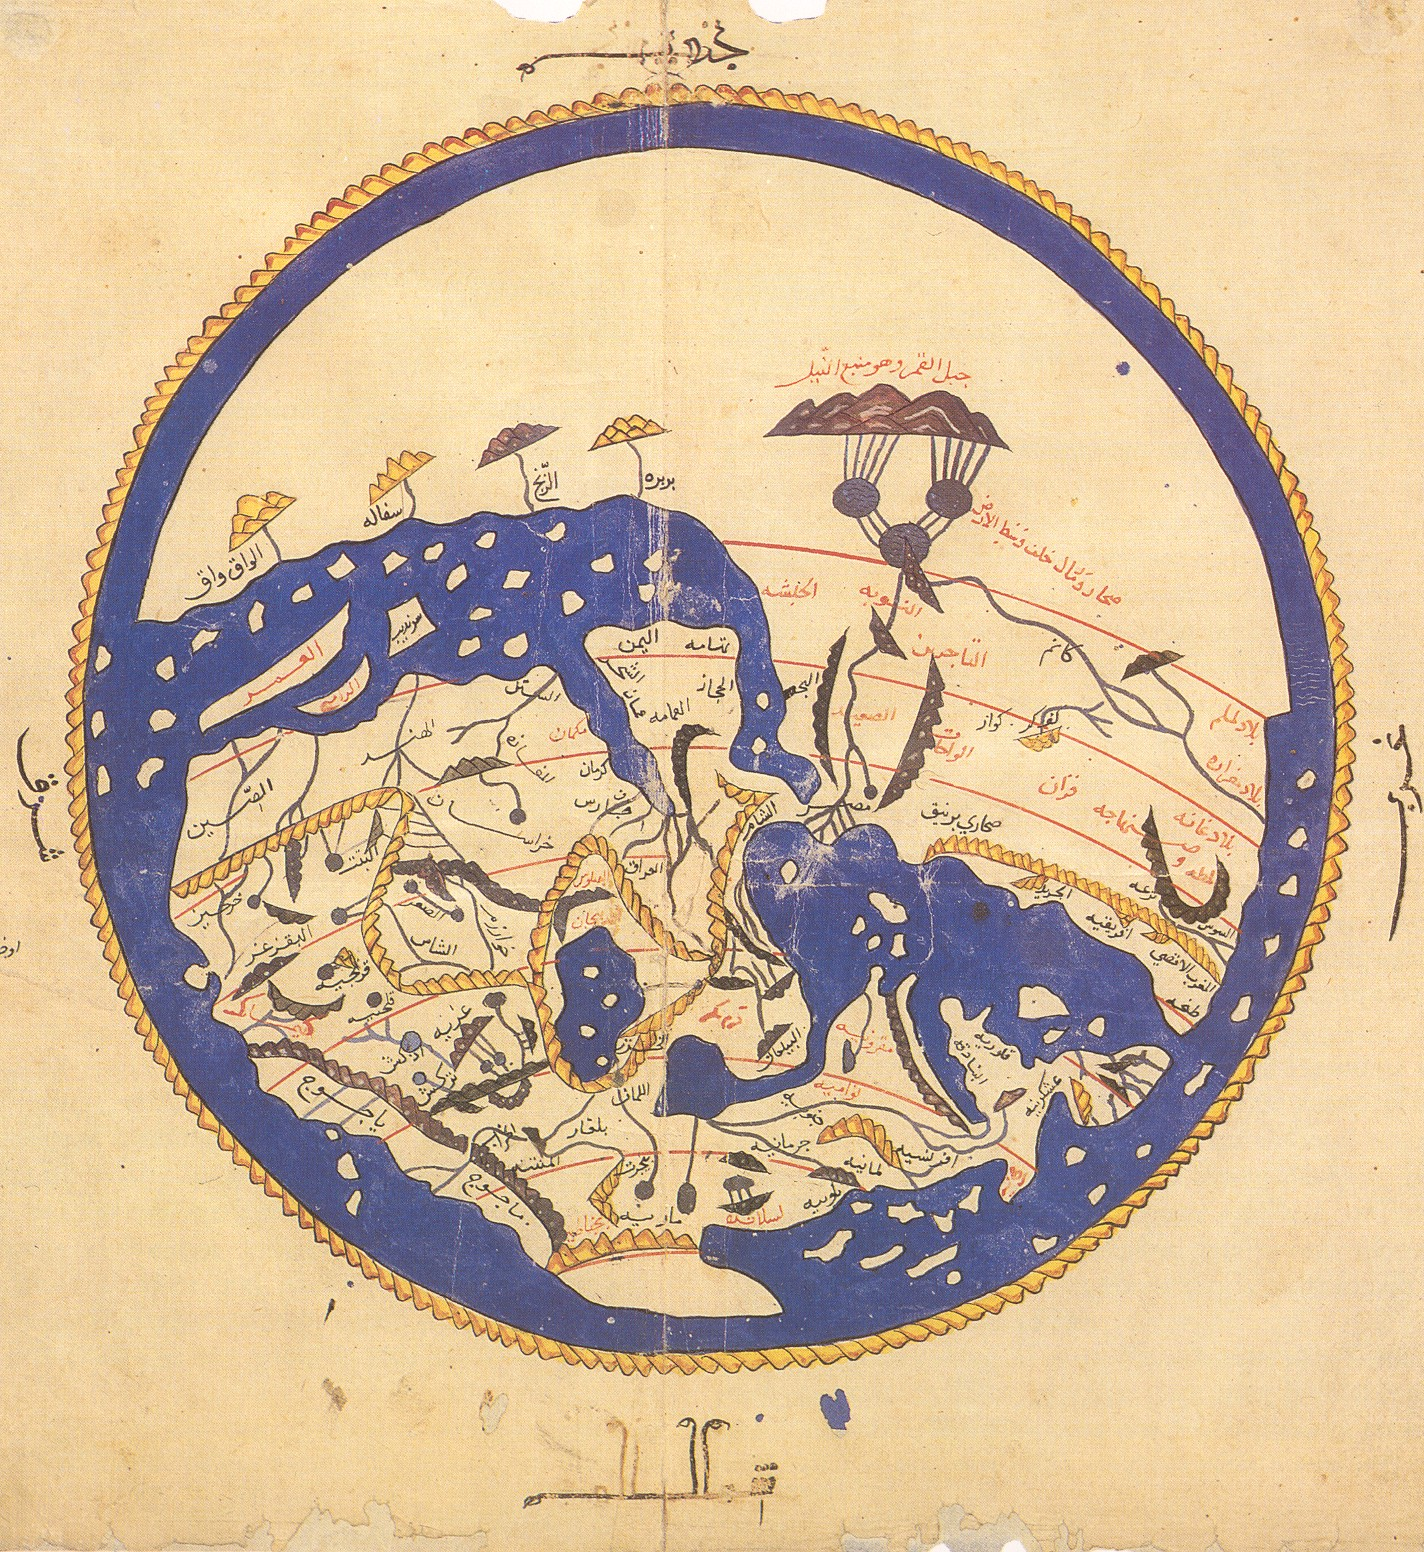
\includegraphics[width=1\textwidth]{figures/petaduniaalid.JPG}}
\caption{Gambaran pengantar peta dunia karya al-Idrisi tahun 1154.}
\end{figure}

\begin{figure}[ht]
	\centerline{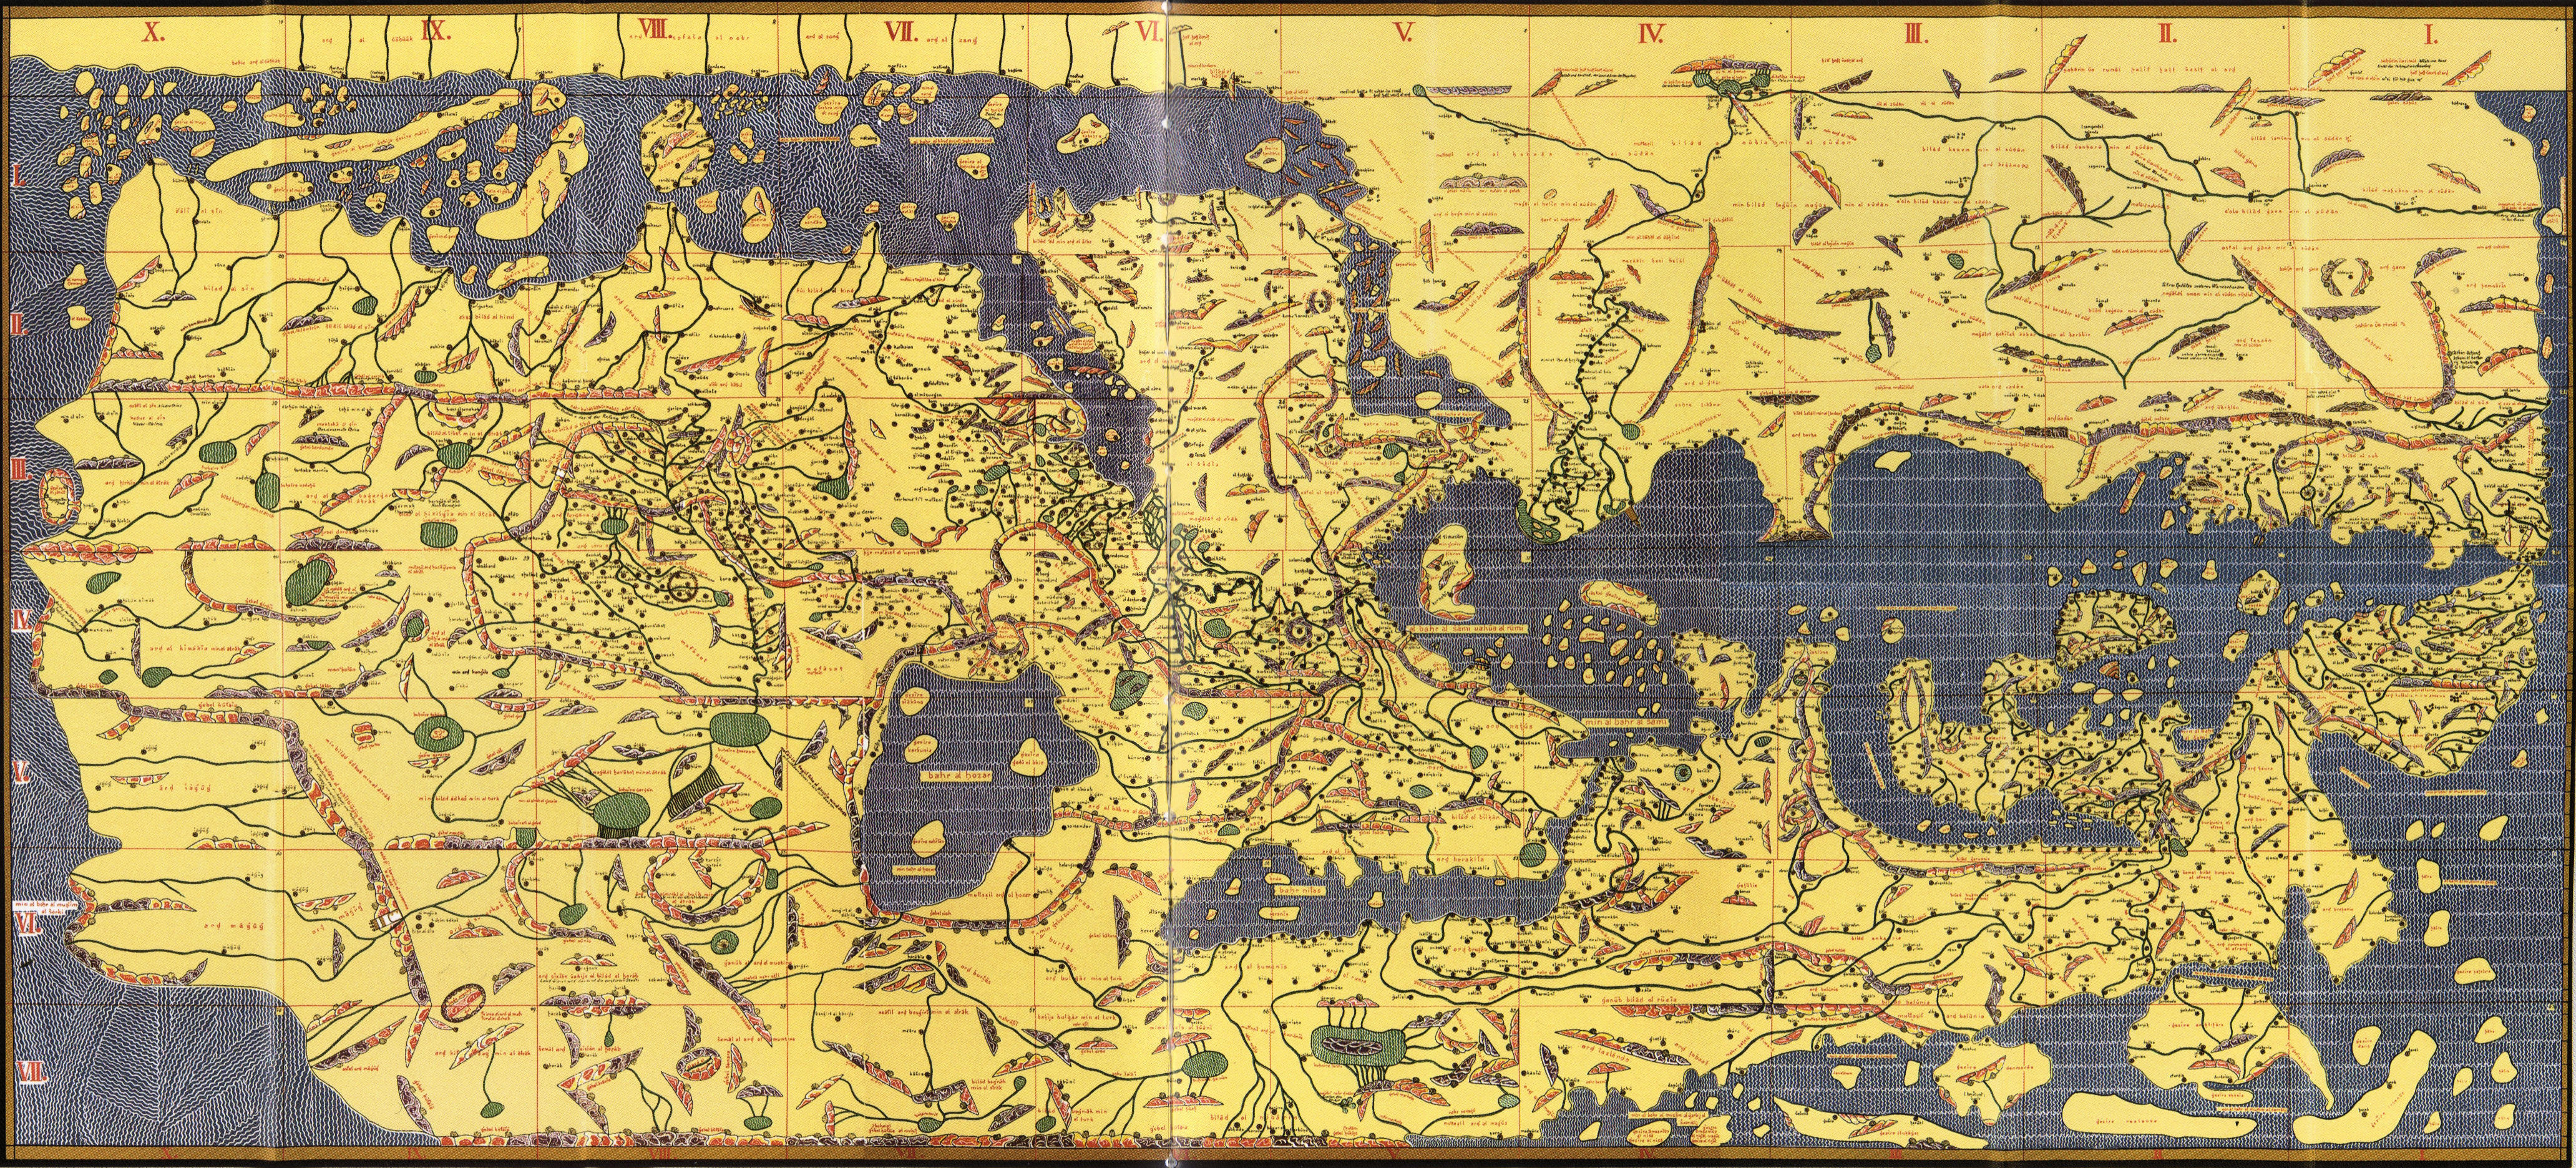
\includegraphics[width=1\textwidth]{figures/TabulaRogeriana.jpg}}
\vskip2pt
\caption{Tabula Rogeriana digambar oleh Al-Idrisi pada tahun 1154 untuk Raja Normandia Roger II dari Sisilia, setelah delapan menetap di istananya, di mana dia bekerja untuk penjelasan dan ilustrasi peta.}
\end{figure}

\section{Penentuan Kordinat}
Kordinat digunakan untuk mengacu sebuah titik lokasi di muka bumi, adapun beberapa jenis standar kordinat yang digunakan adalah.

\subsection{Kordinat Internasional}
Kordinat internasional dikenal dengan long dan lat.


\subsection{Kordinat Indonesia}
Masih ingatkah pelajaran geografi tentang letak Indonesia? maka kita bisa melihat jawaban tersebut dalam kordinat berbahasa indonesia.



\chapter[Pendahuluan]
{Pendahuluan\\ definisi}
% kelompok definisi
% ariana setiawan (1154042)
% idang mawardi (1154084)
% arya niken manalu (1154080)
% M. Arya Sikumbang (1154075)
% r rifa fauzi komara (1154089)
% Andi Tenri Wali (1154013)

\section{Definisi GIS (GEOGRAPHICS INFORMATION SYSTEM)}
Geographical information system (GIS) adalah sebuah komputer yang berbasis sistem
informasi digunakan untuk memberikan informasi bentuk digital dan analisa terhadap 
permukaan geografi bumi.

\subsection{Pemahaman pada Geographics Information System GIS}
Dimana GIS merupakan pemahaman dari, sebagai berikut:
\begin{enumerate}
\item Geography

Dimana GIS dibangun berdasarkan pada istilah‘geografi’ atau ‘spasial’.
Object mengacu pada spesifikasi lokasi dalam suatu tempat/ruang. Objek dapat berupa fisik,
budaya ataupun ekonomi alamiah. Penampakan yang seperti ini ditampilkan pada suatu peta yang 
digunakan untuk memberikan gambaran yang lebih representatif dari spasial dari suatu objek.
sesuai dengan kenyataannya yang di bumi. Dimana simbol, warna dan gaya garis digunakan sebagai
perwakilan dari setiap spasial yang berbeda pada peta dua dimensi.
Pada gambar \ref{dataspasial} dijelaskan bahwa data spasial berikut berupa 
titik, garis, poligon (2-D) dan permukaan (3-D).

\begin{figure}[ht]
	\centerline{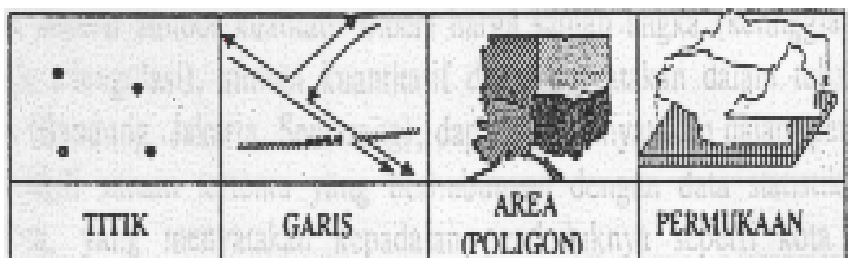
\includegraphics[width=1\textwidth]{figures/dataspasial.JPEG}}
	\caption{data spasial berikut berupa titik, garis, poligon (2-D), permukaan (3-D).}
	\label{dataspasial}
	\end{figure}

Dan arti dari gambar diatas adalah :
Format Titik 						
- Memiliki koordinat tunggal 		
- Tanpa memiliki panjang 			
- Tanpa memiliki luasan

Format Garis
- memiliki koordinat titik awal dan akhir		
- memiliki panjang tanpa luasan

Format Poligon 					
- memiliki koordinat titik awal dan akhir
-memiliki panjang dan luasan 		

Format Permukaan
- memiliki area koordinat vertikal
- memiliki area dengan ketinggian

\item Information
Informasi berasal dari kata pengolahan sejumlah data. Di dalam GIS informasi mempunyai
volume terbesar. Dan setiap object geografi memiliki setting datanya tersendiri karena 
tidak sepenuhnya data yang ada dapat terwakili didalam peta. Maka, semua data harus
diasosiasikan pada objek spasial yang mampu membuat peta menjadi intelligent.

\item System
Pengertian dari suatu sistem merupakan kumpulan elemen-elemen yang saling berintegrasi 
dan berinterdependensi dalam sebuah lingkungan yang dinamis untuk mencapai tujuan tertentu.
\end{enumerate}

\subsection{Definisi GIS (Geography Information and System)}
Dan defenisi dari GIS dapat selalu berubah karena GIS adalah bidang kajian ilmu 
dan teknologi yang masih baru. Beberapa defenisi dari Geographical Information System yaitu:
\begin{enumerate}
\item Definisi GIS menurut(Rhind, 1988):
yaitu : GIS is a computer system for collecting, checking, integrating and analyzing
information related to the surface of the earth.

\item Definisi GIS menurut(Marble \& Peuquet, 1983) and (Parker,
1988; Ozemoy et al., 1981; Burrough, 1986):
yaitu : GIS deals with space-time data and often but not necessarily, employs computer
hardware and software.

\item Difinisi GIS menurut (Purwadhi, 1994):
- SIG adalah suatu sistem yang mampu mengorganisir perangkat keras (hardware),
perangkat lunak (software), dan data, serta dapat mendaya dan digunakan sistem
penyimpanan, pengolahan, maupun analisis data yang dilakukan secara simultan, sehingga dapat
diperoleh seluruh informasi yang berkaitan secara langsung dengan aspek keruangan.
- SIG adalah manajemen data spasial dan data non-spasial yang berbasis komputer
dengan menggunakan tiga karakteristik dasar, yaitu: 
(i) memiliki fenomena yang aktual (variabel data non-lokasi) dan berhubungan 
dengan topik permasalahan di lokasi bersangkutan; 
(ii) merupakan suatu kejadian di suatu lokasi tertentu; 
(iii) memiliki dimensi waktu. Alasan GIS dibutuhkan adalah karena untuk data spasial 
penanganannya sangat sulit karena peta dan data statistik cepat mengalami kadaluarsa 
sehingga tidak ada pelayanan penyediaan data dan informasi yang diberikan menjadi tidak akurat.
\end{enumerate} 

Berikut merupakan keistimewaan analisa dengan Geographical Information System (GIS) yaitu:
\begin{enumerate}
\item Analisa Proximity
Analisa Proximity adalah geografi yang berbasis pada jarak antar layer.
Didalam analisis proximity GIS menggunakan proses yang disebut dengan buffering
yaitu membangun lapisan pendukung sekitar layer dalam jarak tertentu agar dapat menentukan
dekatnya hugungan antara sifat bagian yang ada.
\item Analisa Overlay
Analisa Overlay adalah proses integrasi data dari lapisan-lapisan layer yang berbeda (overlay).
Yang secara analisa membutuhkan lebih dari satu layer yang akan ditumpang susun secara
fisik agar dapat dianalisa secara visual.
\end{enumerate}

Maka artikel :
	Dalam sebuah artikel dari husein yang menyebutkan bahwa  GIS merupakan pemahaman dari
	Geography, Information dan System \cite{husein2006konsep}.

\section{Geographic Information System (GIS): Introduction to the computer perspective}
Sistem Informasi Geografi (GIS) diartikan sebagai sistem untuk menyimpan, memeriksa, 
mengintegrasi, memanipulasi, menganalisis dan memaparkan data yang berkaitan dengan semua 
ruang yang berhubungan dengan keadaan bumi.
Maka artikel :
	Dalam sebuah artikel dari prahasta yang menyebutkan bahwa  GIS merupakan menyimpan, memeriksa, mengintegrasi, memanipulasi, menganalisis dan memaparkan data yang berkaitan dengan semua ruang yang berhubungan dengan keadaan bumi., Information dan System \cite{prahasta2009sistem}.

\subsection{Pengenalan GIS atau Geography Information System}
1. GIS atau dikenal dengan Sistem Informasi Geografi ditunjukan sebagai sistem yang mampu menyimpan, memeriksa, mengintegrasikan, memanipulasi, menganalisis dan memaparkan data-data yang terkait dengan spasial yang merunjuk terhadap bagian bumi. (Jabatan Alam Sekitar, 1987).

2. GIS merupakan satu set lat untuk mengumpulkan, menyimpan, mendapatkan, mengubah dan memaparkan data ruang dari keadaan  bumi yang sebenarnya untuk keperluan tertentu (Burrough, 1986).

3. GIS adalah setiap set manual atau prosedur komputer yang digunakan untuk menyimpan dan memanipulasi data geografis yang tersedia (Arronoff, 1989).

4. GIS merangkum keadaan bumi dengan peranti atau perangkat tertentu yang digunakan untuk peta input atau peta produk, bersama-sama dengan dengan sistem komunikasi yang diperlukan untuk dijadikan sebagai penghubung berbagai unsur. (Star \& Ester, 1990).

5. GIS adalah suatu sistem untuk membantu dalam membangunkan model tertentu yang mustahil untuk dijadikan sintesi data yang banyak. (Martin, 1996).

\subsection{Komponen GIS atau Geography Information System}
Komponen GIS sendiri dibagikan menjadi 3 komponen, yaitu :
Sistem Komputer (perkakas dan sistem operasi), Software GIS
(ArcGIS), database GIS, methode GIS (Prosedur analisis), People (Orang-orang yang menggunakan GIS/User).
Pada gambar \ref{komponenGIS} dijelaskan bahwa kompnen GIS sebagai berikut.

\begin{figure}[ht]
	\centerline{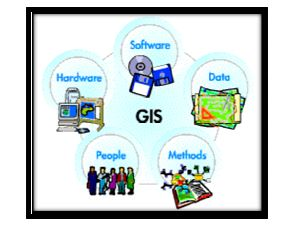
\includegraphics[width=1\textwidth]{figures/komponenGIS.JPG}}
	\caption{komponen GIS.}
	\label{komponenGIS}
	\end{figure}

\subsubsection{Komponen GIS atau Geography Information System}
sesuai dengan gambar diatas komponen GIS dibagi menjadi 3 bagian, yaitu :
1. Sistem Komputer (perkakas dan sistem operasi), merupakan hardware dari sebuah sistem GIS. Perkakas terdiri dari monitor, unit sistem atau CPU, keyboard dan mouse (Heywood et al., 2002). Teknologi komputer harus memiliki kemampuan kuasa
yang tinggi untuk menjalankan perisian GIS.

2. Software GIS , merupakan ArcGIS untuk tujuan perancangan, pengurusan ataupun pemodelan pada kebutuhan tertentu.

3. Database GIS , merupakan tempat yang melibatkan data GIS baik data spatial dan pengurusan datanya. memori untuk menyimpan jumlah data yang besar dan mempunyai kualitas yang baik dengan resolusi tinggi pada skrin grafik warna (untuk membantu dalam menentukan maklumat yang dihasilkan atau diberikan melalui penggunaan warna yang berbeda).

4. Methode GIS , merupakan prosedur dari analisis sistem GIS. yang melibatkan proses input, proses menyimpan, proses mengurus, proses menukar, proses menganalisis, dan proses output yang hanya melibatkan perisian GIS untuk mengatur sistem dan data-data tersebut (Heywood et al., 2002 )

5. People , merupakan orang-orang yang menggunakan sistem GIS. atau orang yang mengendaliakn proses input-output sistem GIS. 

\subsection{Kaedah GIS atau Geography Information System}
Berdasarkan pemahaman diatas, kaedah GIS juga merupakan salah satu komponen penting untuk mengatur sistem GIS sesuai dengan penjelasan sebelumnya. Kaedah-kaedah ini terdiri dari input
data spatial, pengurusan data atribut, paparan data, penerokaan data, analisis dan pemodelan data GIS;
yang dijelaskan oleh gambar sebagai berikut:
Pada gambar \ref{kaedahGIS} dijelaskan bahwa kaedah GIS sebagai berikut.
\begin{figure}[ht]
	\centerline{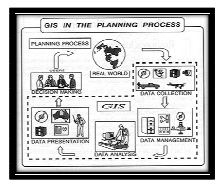
\includegraphics[width=1\textwidth]{figures/kaedahGIS.JPG}}
	\caption{kaedah GIS.}
	\label{kaedahGIS}
	\end{figure}

\subsubsection{Kaedah GIS atau Geography Information System}
1. Input data spatial
Merupakan langkah awal agar terciptanya data baru, dengan cara menginputkan data dan sistem GIS akan menyuntingnya dalam bentuk transformasi geometri yang nantinya akan menghasilkannya kedalam bentuk hard copy. (Chang, 2008) 
(Heywood et al., 2002).

2. Pengurusan data artibut
Merupakan langkah selanjutnya agar sumber peta dapat dipindahkan kepada peta digital yang dapat dibaca oleh GIS.
(Chang, 2008) (Worboy \& Duckham, 2003) (Heywood et al., 2002)

3. Pengumpulan data
Merupakan aktivitas untuk proses melakukan eksplorasi lebih jauh dalam meneliti ciri kesamaa dalam suatu graf peta yang berbeda. (Worboy \& Duckham, 2003).

4. Analisis data
Merupakan cara untuk memaparkan dan memanipulasi data yang didapat. Dengan menggunakan 2 jenis format, yaitu :
- data vektor : melibatkan beberapa kaedah seperti penimbalan / buffering, penindihan/overlay, pengukuran jarak, statik ruang, dan manipulasi peta.
- data raster : menaganalisis pengumpulan data tempatan, kaedah kejiranan, kaedah berzon, dan kaedah operasi global.
(Chang, 2008) (Worboy \& Duckham, 2003) (Heywood et al., 2002)

5. Paparan data dan output data
Dasarnya disediakan untuk tujuan pemaparan hasil dari analisis data yang fungsinya ditujukan untuk pengguna.

6. Aplikasi GIS
Digunakan untuk keperluan tertentu dan bersifat umum bagi masyarakat tergantung keperluan penggunanya. 
(Heywood et al., 2002).

Pada gambar \ref{aplikasiGIS} dijelaskan bahwa aplikasi GIS sesuai keperluan penggunan sebagai berikut.
\begin{figure}[ht]
	\centerline{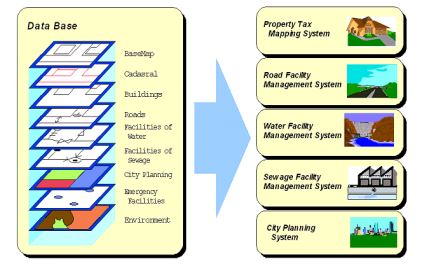
\includegraphics[width=1\textwidth]{figures/aplikasiGIS.JPG}}
	\caption{aplikasi GIS.}
	\label{aplikasiGIS}
	\end{figure}
Maka artikel :
	Dalam sebuah artikel dari hua yang menyebutkan bahwa  GIS memiliki kaedah dan komponen, Information dan System \cite{hua2017sistem}.

\subsection{Kesimpulan GIS atau Geography Information System}
Kesimpulannya, GIS merupakan alat yang penting dalam perspektif komputer pada masa kini dikarenakan GIS
mempunyai kemampuan aplikasi dalam berbagai bidang, misalnya dalam proses perancangan bandar dan kartografi,
penilaian kesan alam sekitar dan pengurusan sumber asli. GIS juga memainkan peranan dalam perspektif perniagaan,
dimana alat ini sangat bermanfaat dalam pengiklanan dan pemasaran, jualan, dan logistik 
mampu digunakan untuk mencari dan meningkatkan perniagaan seperti tapak perniagaan yang strategik. Sebagai umum, pengguna GIS dapat dilibatkan dengan agensi-agensi penguatkuasaan undang-undang, strategi
perancangan, perhutanan, industri, pemberdayaan alam, perencanaan kota, profesional
telekomunikasi, kesehatan, pengangkutan, geografi, dan pembangunan pemasaran. 
Penjelasan ini menyediakan platform untuk memahami lebih lanjut tentang komponen, kaedah, dan aplikasi GIS, 
untuk mempelajari tentang alat GIS.
\subsection{Saran GIS atau Geography Information System}
GIS dapat diaplikasikan di dalam kehidupan sehari-hari untuk memenuhi kebutuhan dan dapat membantu kebutuhan setiap masyarakat menjadi lebih baik dan lebih bermanfaat. Karena dengan memanfaatkan kemajuan teknologi maka teknologi yang digunakan akan ikut turut serta terus perkembang untuk menyesuaikan pemenuhan kebutuhan setiap pengguna yaitu masyarakat. Demikian kesimpulan dan saran yang dapat disampaikan kurang lebihnya mohon maaf dan terimakasih.

\subsection{SIG mempresentasikan real world dengan data spasial yang terbagi atas 2 model data, yaitu:}
1. Vektor, Bumi dalam data vector direpresentasikan sebagai mozaik yang terdiri atas garis, polygon, titik,
dan noders.
Model data vector merupakan model data yang paling banyak digunakan, model ini berbasiskan
pada titik dengan koordinat (x,y) untuk membangun objek spasialnya. Objek yang dibangun
dibagi menjadi tiga bagian, yaitu: titik, garis, dan area (polygon).
Keuntungan dari data vector, yaitu: ketepatan dalam merepresentasikan fitur titik, batasan dan
garis lurus.
2. Raster, Data raster adalah data yang dihasilkan dari sistem pengindraan yang jauh. Pada data raster,
objek geografis direpresentasikan sebagai struktur sel grid yang disebut pixel. Resolusi pada data
raster tergantung pada ukuran pixel-nya.
Maka, resolusi pixel menggambarkan ukuran sebenarnya dari permukaan bumi yang diwakili
oleh setiap pixel pada citra. Semakin tinggi resolusinya, semakin kecil permukaan bumi yang
direpresentasikan oleh suatu sel. Data raster cocok untuk merepresentasikan batas-batas yang
berubah secara gradual, seperti jenis tanah, vegetasi, suhu tanah, dan kelembaban tanah.


\chapter[Bangun Ruang]
{Pengantar\\ Bangun Ruang}
%kelompok 2
%Achmad Fatahillah(1154004)
%Ilga Anne Tri J.S(1154045)
%Maulyanda(1154008)
%Mefi Frinkazela Nikica(1154073)
%Simon Sorba Manangi(1154019)
	
\section{Bangun Ruang}
Bangun ruang merupakan suatu bagian ruang yang dibatasi oleh himpunan titik-titik yang terdapat pada seluruh permukaan bangun tersebut. 
Permukaan bangun tersebut disebut sisi. Bangun ruang memiliki tiga unsur, yaitu 
panjang : merupakan suatu dimensi dalam benda yang menunjukkan sebuah jarak antar ujung satu ke ujung lainnya.
lebar   : merupakan lintasan dalam sebuah bidang.
tinggi  : merupakan ukuran sebuah objek yang diukur secara vertikal.
Bangun ruang memiliki volume. Rumus volume umum pada bangun ruang adalah panjang(p) x lebar(l) x tinggi(t).
Tujuan menghitung volume adalah untuk menghitung berapa banyak ruang yang dapat diisi datau ditempati pada suatu objek.

Sisi bangun ruang adalah suatu himpunan pada titik-titik yang terdapat pada permukaan atau yang membatasi suatu bangun ruang tersebut \cite{umami2013eksperimentasi}

Dalam memilih model untuk permukaan atau sisi, dapat karena kedudukan semua unsur bangun ruang dapat diamati untuk dialihkan dalam gambar\cite{suharjana2008mengenal}. 
Ada beberapa contoh benda yang mewakili gambar bangun ruang\ref{contohbangun}.
\begin{figure}[ht]
    \centerline{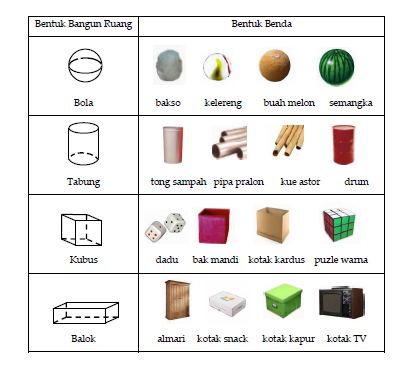
\includegraphics[width=1\textwidth]{figures/contohbangun.png}}
    \caption{beberapa kumpulan gambar yang termasuk dalam bangun ruang}
    \label{contohbangun}
    \end{figure}
 
Bangun ruang sering  disebut bangun 3 dimensi karena memiliki 3 komponen utama sebagai berikut.
1.Sisi  merupakan bidang pada bangun ini memiliki ruang yang membatasi antara bangun ruang dengan ruangansekitarnya 
2.Rusuk merupakan pertemuan antar dua sisi yang berupa ruas garis pada bangun.
3.Titik sudut merupakan titik hasil pertemuan rusuk yang berjumlah tiga atau lebih

Unsur-unsur Bangun Ruang Sisi,rusuk,dantitiksudut. Sebagai mengingatkan bahwa setiap model bangun ruang pasti memiliki sisi, rusuk, dan titiksudut , kecuali bola, tabung,dankerucut.
Bangun ruang, limas, prisma, dan sisi, rusuk, titiksudut serta dikembangkan pada diagonalsisi,diagonalruang, dangaris-garis sejajar.
menggunakan model bangun ruang yang transparan  melihat sisi bangun ruang tersebut, model transparan, bangun ruang dengan model transparan ini juga dapat untuk menggambar bangun ruang, karena semua unsur bangun ruang dapat diamati untuk dialihkan dalam gambar. Setelah mengamati, 
menelusuri, dan memahami unsur-unsur bangun ruang tersebut.

Jenis-Jenis Bangun Ruang yang umum dikenal adalah:
1.  kubus merupakan bangun ruang yang dibatasi oleh enam buah bidang sisi berbentuk persegi dengan ukuran yang sama.
2.balok yaitu bangun ruang dengan dibatasi dengan enam bidang sisi yang memiliki bentuk persegi panjang yang setiap sepasang-sepasang sejajar dan sama ukurannya.
3.prisma yaitu adalah sebuah bangun ruang yang diberikan batas oleh dua buah daerah segitiga yang sejajar sehingga tiga daerah persegi panjang tersebut yang saling berpotongan menurut garis-garis yang sejajar.
4.limas merupakan bangun ruang yang dibatasi leh sebuah daerah segiempat dan empat daerah segitiga yang mempunyai satu titik sudut persekutuan.
5.kerucut merupakan bangun ruang yang dibatasi oleh sebuah bidang lengkung yang simetris terhadap porosnya yang melalui titik pusat lingkaran tersebut.
6.tabung merupakan bangun ruang yang setiap sisinya dibatasin dengan dua bidang lingkaran yang sama-sama sejajar dan sama-sama ukurannya dan satu buah bidang 
     yang memiliki jarak sama jauhnya ke arah poros dan sisi yang simetris ke arah porosnye itu akan memotong dua daerah bidang lingkaran tepat di kedua lingkaran itu .
7.Bola
Jenis-Jenis Bangun Ruang yang umum dikenal adalah dan di dalam kehidupan sehari hari:
1.   Kubus    : dadu, rubik
2.   Balok    : lemari, tv
3.   Prisma    : atap rumah, tenda pramuka
4.   Limas    : piramida, monas
5.   Kerucut: nasi tumppeng yang berbentuk kerucut
6.   Tabung    : minuman kaleng, gas elpiji
7.   Bola    : bola basket, bola tenis

Dalam pembelajaran bangun ruang dan unsur-unsurnya maka harus DIPERKENALKAN model-model bangun ruang, misalnya model kubus, balok, prisma, limas, tabung, kerucut, dan bola. apabila diambil contoh-contoh dari bendabenda yang dapat ditemukan dalam kehidupan sehari-hari, misalnya kaleng roti untuk menunjukkan tabung, tumpeng untuk menunjukkan kerucut dan seterusnya. Yang tidak transparan, transparan dan kerangka. Hal tersebut akan lebih memudahkan dalam pemahamanbangun ruang dan unsur unsurnya, menentukan sifat sifat bangun ruang, serta dapat menterjemahkan gambar dalam bangun ruang dans ebaliknya.
Contoh di bidang bangun ruang yaitu dalam bidang geometri  materi matematika bentuk bangun datar 2D maupun bangun ruang 3D. 
Manfaat yang dapat diperoleh dari penelitian memberikan gambaran 3D dari pemodelan bangun geometri halnya alat perga dalam membangun siswa dalam mempelajari bentuk bangun geometri.
Bangun ruang dalam bentuk geometris yang terdiri atas tiga dimensi( panjang lebar dan tinggi) bangun ruang yang di bahas di dalam geometri antara lain :
1.    Kubus
2.    Balok 
3.    Prisma
4.    Limas
5.    Tabung
6.    Kerucut
7.    Bola

Kebutuhan di bangun ruang dapat disimpulkan bahwa diperlukan 
1.    Pengertian dan ciri-ciri berapa bangun datar dan bangunan ruangan.
2.    Data rumus luas bangun datar.
3.    Data rumus volum bangun datar dan bangun ruang.

Kebutuhan disini sudah diperoleh dari buku matematika sekolah dasar.

\subsection{Bola} 

\begin{figure}[ht]
    \centering
	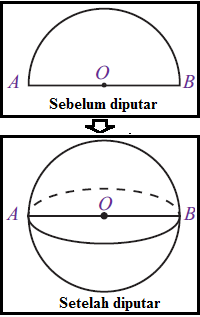
\includegraphics[width=0.5\textwidth]{figures/bola1.png}
    \caption{contoh bola}
    \label{bola1}
\end{figure}

Dalam bangun ruang, bola adalah bangun ruang tiga dimensi yang dibentuk sehingga tak terhingga lingkaran yang berjari-jari sama panjangnya dan berpusat pada satu titik yang sama. Bola merupakan bangun ruang sisi lengkung yang dibatasi oleh satu bidang lengkung.
contoh bangun ruang bola dalam kehidupan sehari-hari adalah dalam sebuah olah raga sepak bola, basket, kasti, bowling, dan sebagai nya. bola dapat menggelinding dan dapat memantul dengan sempurna, karena tidak adanya sudut pada bola. 
Bentuk bumi pun seperti bola, terlihat pada sebuah dokumentasi dari pesawat ruang angkasa, maupun dalam hal perjalan lurus, pasti akan kembali lagi ketempat kita memulai perjalanan.
Bola dapat dibentuk dari bangun setengah lingkaran yang diputar sejauh 360° pada garis tengahnya. 
Pada gambar  \ref{bola1} merupakan setengah lingkaran dengan diameter AB  tersebut dan dapat diputar satu putaran dengan diameter sebagai suatu sumbu putar maka akan tampak gambar seperti di bawahnya yang disebut bangun ruang.


Bola merupakan bangun ruang sisi lengkung (BRSL) yang terjadi dari tumpukan empat buah lingkaran \ref{sisilengkung}.
\begin{figure}[ht]
    \centering
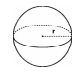
\includegraphics[width=0.25\textwidth]{figures/sisilengkung.png}
    \caption{contoh sisi lengkung}
    \label{sisilengkung}
    \end{figure} 
Keempat lingkaran ini dinamakan kulit bola. Kulit bola berada pada sisi luar bola atau mengelilingi bola \cite{nurfarikhin2010hubungan}.

Rumus bola:

a) Luas permukaan
 \begin{equation}
     L = 4 \pi r^2 \,
\end{equation}
b) Volume
\begin{equation}
     V = \frac{4}{3}\pi r^3
\end{equation}
\subsubsection{Sifat-sifat pada bola} 
a) Memiliki 1 sisi yang berbentuk bidang lengkung (selimut bola) 
b) Tidak memiliki rusuk 
c) Tidak memiliki titik sudut
 
Adapun unsur-unsur bangun ruang bola yang terdapat pada gambar \ref{unsurbola} sebagai berikut.
\begin{figure}[ht]
    \centerline{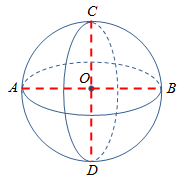
\includegraphics[width=1\textwidth]{figures/unsurbola.png}}
    \caption{contoh usur bola}
    \label{unsurbola}
    \end{figure}
1) Titik pada titik O dinamakan titik pusat bola.
2) Ruas garis pada OA disebut sebagai jari-jari pada bola. Sebutkan jari-jari pada bola lainnya.
3) Ruas garis pada CD diberi nama sebagai diameter pada bola. Jika kita amati, ruas pada garis AB tersebut merupakan diameter bola. AB dapat pula disebut sebagai tinggi bola.
4) Sisi bola merupakan kumpulan titik - titik yang mempunyai jarak yang sama terhadap titik O. Sisi tersebut dinamakan selimutatau kulit bola.
5) Ruas garis ACB dinamakan tali busur bola.
6) Ruas-ruas pada garis selimut bola yaitu ACBDA dinamakan garis pelukis bola.

\subsubsection{Konsep luas permukaan Bola}
Penentuan luas sisis (permukaan) bola dapat kita lakukan dengan sebuah percobaan archimedes, yaitu:
Sebuah bola menempati sebuah tabung yang memiliki diameter dan tinggi tabung sama tepat dengan 
yang dimiliki oleh diameter bola, maka luas bola itu sama dengan luas selimut tabung \ref{bolatabung}.
\begin{figure}[ht]
    \centerline{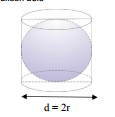
\includegraphics[width=1\textwidth]{figures/bolatabung.png}}
    \caption{sebuah bola yang terdapat dalam tabung, untuk mengukur luar permukaan tabung}
    \label{bolatabung}
    \end{figure} 
Berdasarkan gambar maka diperoleh :

Luas selimut tabung 
\begin{equation}
					L= 2 pr. T
                    = 2pr. 2r
                    = 4pr2
\end{equation}
            
\subsubsection{Konsep volume bola}
Apabila kita mengisi air ke dalam bangun bola secara penuh 
kemudian menuangkannya ke bangun ruang tabung maka air yang diperoleh adalah 2/3 bagian dari volume bangun ruang tabung tersebut. 
Dengan ketentuan bahwa kedua bangun tersebut memiliki jari-jari yang sama sehingga diperoleh:
\begin{equation}
Volume bola = 2/3 . volume tabung(silinder)
            = 2/3 . (pr2 . 2r)
\end{equation}

\subsubsection{Asal-usul rumus permukaan bola}
Jika ingin mendapatkan rumus permukaan bola, kita mulai kegiatan berikut ini untuk menguji rumus tersebut.
1. Sediakan sebuah bola berukuran sedang seperti bola sepak atau bola basket.
2. Ukurlah setiap keliling bola tersebut menggunakan benang.
3. Lilitkan benang tersebut pada permukaan setengah bola sampai penuh, seperti gambar \ref{bola2}.
\begin{figure}[ht]
    \centerline{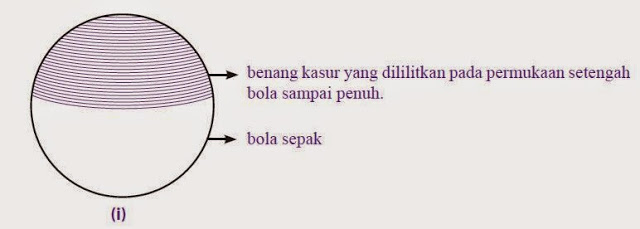
\includegraphics[width=1\textwidth]{figures/bola2.jpg}}
    \caption{gambar bola}
    \label{bola2}
    \end{figure}
4. Buatlah persegi panjang dari kertas karton dengan ukuran panjang sama dengan keliling bola dan lebar sama dengan diameter bola seperti gambar \ref{bola3}.
\begin{figure}[ht]
    \centerline{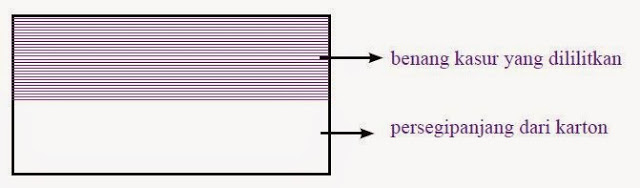
\includegraphics[width=1\textwidth]{figures/bola3.jpg}}
    \caption{beberapa kumpulan gambar yang termasuk dalam bangun ruang}
    \label{bola3}
    \end{figure}
5. Lilitkan benang yang telah digunakan untuk melilit permukaan setengah bola pada persegipanjang yang kamu buat tadi. Lilitkan sampai habis.
6. Jika kamu melakukannya dengan baik, tampak benang tersebut menutupi persegi panjang selebar jari-jari bola (r).
7. Hitunglah luas dari persegi panjang yang telah ditutupi benang tersebut. 
\begin{equation}
Luas permukaan setengah bola = luas persegi panjang
                                           = p × l
                                           = 2πr× r
                                           = 2π r2
\end{equation}

Jadi, luas permukaan bola dirumuskan sebagai berikut :
\begin{equation}
Luas permukaan bola ( L = 4πr2 )
\end{equation}
Keterangan :
L = luas permukaan bola.
r = jari-jari bola.
π = 22/7 atau 3,14

\subsubsection{Asal-usul rumus volume bola}
Cara - cara untuk mengetahui rumus volume bola, dapat dilakukan dengan cara - cara seperti berikut ini : 
1. Siapkan sebuah tempat yang berbentuk setengah bola berjari-jari r (\ref{wadah1}) dan sebuah wadah yang berbentuk kerucut berjari-jari r dan tingginya 2r (\ref{wadah2}).
2. Isikan pasir ke \ref{wadah2} sampai penuh.
3. Pindahkan pasir di dalam \ref{wadah2} ke \ref{wadah1}. Apakah yang terjadi?
\begin{figure}[ht]
    \centerline{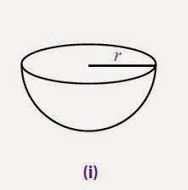
\includegraphics[width=1\textwidth]{figures/wadah1.jpg}}
    \caption{wadah dalam bola}
    \label{wadah1}
    \end{figure}
\begin{figure}[ht]
    \centerline{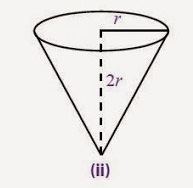
\includegraphics[width=1\textwidth]{figures/wadah2.jpg}}
    \caption{pasir dalam wadah}
    \label{wadah2}
    \end{figure}

Dari cara seperti diatas tersebut, dapat dilihat bahwasanya volume dari pasir yang dituangkan ke dalam wadah setengah bola tidak dapat berubah. Ini berarti, untuk membangun setengah bola, dan kerucut yang berjari-jari sama, dan tinggi kerucut sama dengan dua kali jari-jarinya maka:
\begin{equation}
Volume setengah bola = volume kerucut
1/2 volume bola = 1/3 πr2t
volume bola = 2/3πr2(2r)
                         = 4/3πr3
\end{equation}
Jadi, volume bola tersebut dirumuskan sebagai berikut :
\begin{equation}
Volume bola ( V = 4/3πr3 )
\end{equation}
Keterangan :
V = volume bola.
r = jari-jari bola.
π =22/7 atau 3,14.

Contoh soal :
bola memiliki jari-jari 9 cm, hitunglah volume bola tersebut ?

Jawab :
Diketahui : r = 9 cm
Ditanyakan : volume bola ?
Penyelesaian :
\begin{equation}
V   = 4/3pr3
    = 4/3/ 3 , 14 . (9)3
    = 3.052,08
\end{equation}
Jadi, volume bola tersebut 3.052,08 cm3

\chapter[Diagram Kartesius]
{Pengantar\\ Kartesius}
% Kelompok Diagram Kartesius
% Rahmi Nurdin (1154109)
% Mustari Muammar (1154108)
% Fadillah Firdaus (1154103)

\section{Pengertian Diagram Kartesius}
Diagram Kartesius adalah sistem kooordinat yang terdiri dari dua sumbu yang berisi titik-titik sebagai simbol relasi.
Domain sebagai sumbu horizontal dan kodomain sebagai sumbu vertikal.
Pada koordinat kartesius daerah asal (domain) diletakkan pada sumbu X (sumbu mendatar) dan daerah kawan (kodomain) diletakkan pada sumbu Y (sumbu tegak).
Sedangkan daerah hasilnya merupakan titik (noktah) koordinat pada diagram kartesius. Dari relasi di atas, dapat ditunjukkan diagram kartesiusnya seperti di bawah :
\begin{figure}[ht]
	\centerline{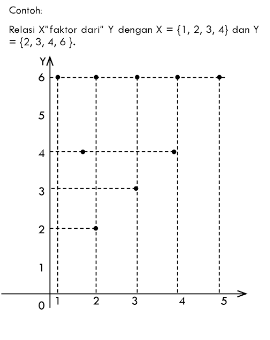
\includegraphics[width=1\textwidth]{figures/rahmi1.PNG}}
	\caption{hubungan antar titik pada diagram kartesius.}
	\label{rahmi1}
	\end{figure}

Diagram Kartesius merupakan suatu bangunan atas empat bagian yang batasi oleh dua buah garis yang berpotongan tegak lurus pada titik-titik (  X, Y ). 
Dimana X merupakan rata-rata dari rata-rata skor tingkat pelaksanaan atau kepuasan konsumen dari sebuah faktor atribut 
dan Y adalah rata-rata skor tingkat kepentingan seluruh faktor atau atribut yang mempengaruhi kepuasan konsumen.
Seluruhnya ada K faktor. Rumus berikutnya yang digunakan adalah :
\begin{figure}[ht]
	\centerline{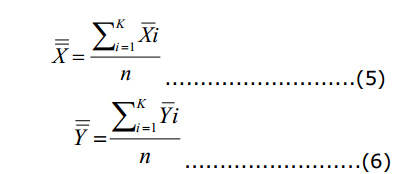
\includegraphics[width=1\textwidth]{figures/rahmi2.PNG}}
	\caption{rumus mencari K faktor.}
	\label{rahmi2}
	\end{figure}

Dimana :K = Banyaknya faktor atau atribut yang mempengaruhi kepuasan konsumen 
Diagram Kartesius	
\begin{figure}[ht]
	\centerline{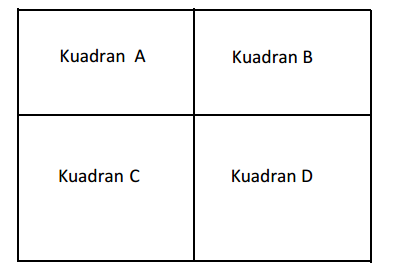
\includegraphics[width=1\textwidth]{figures/rahmi3.PNG}}
	\caption{penentuan kuadran pada diagram kartesius.}
	\label{rahmi3}
	\end{figure}

Gambar 1. Diagram Kartesius



Kuadran A
Pada posisi ini, jika dilihat dari kepentingan konsumen, atribut-atibut produk berada pada tingkat tinggi, tetapi jika di lihat dari kepuasannya, 
konsumen merasakan tingkat yang rendah, sehingga konsumen menuntut adanya perbaikan atribut tersebut.
Kuadran B
Pada posisi ini, jika dilihat dari kepentingan konsumen, atribut-atribut produk berada pada tingkat tinggi, dan dilihat dari kepuasannya, 
konsumen merasakan tingkat yang tinggi juga.
Kuadran C
Pada posisi ini, jika dilihat dari kepentingan konsumen, atribut-atribut produk kurang dianggap penting, tetapi jika dilihat dari tingkat kepuasan konsumen cukup baik.
Namun, konsumen mengabaikan atributatribut yang terletak pada posisi ini.
Kuadran D
Pada posisi ini, jika dilihat dari kepentingan konsumen, atribut-atribut produk kurang dianggap penting, tetapi jika dilihat dari tingkat kepuasanya, konsumen merasa
sangat puas.


\section{Penghitungan Rumus Diagram Kartesius}
\subsection{meghitung rumus, mencari titik}

Kartesius digunakan untuk menentukan tiap titik dalam bidang dengan menggunakan dua bilangan yang biasa disebut koordinat x dan koordinat y.
\begin{figure}[ht]
	\centerline{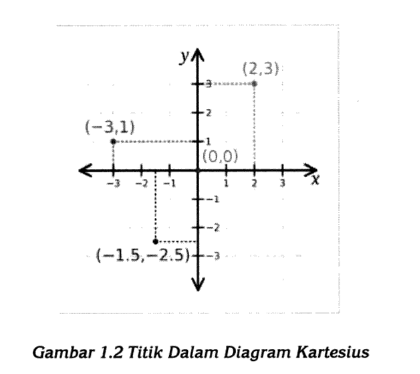
\includegraphics[width=1\textwidth]{figures/rahmi9.PNG}}
	\caption{penentuan titik pada kuadran katesius.}
	\label{rahmi9}
	\end{figure}

Sebuah titik dalam Diagram Kartesius, mengandung dua buah informasi yakni sumbu (x,y), seperti tampak pada Gambar 1.2. 
Yaitu titik (2,3) adalah titik dimana nilai x=2 dan y=3. Daerah ini dikenal dengan kuadran I, dimana nilai x dan y adalah positif.
\begin{figure}[ht]
	\centerline{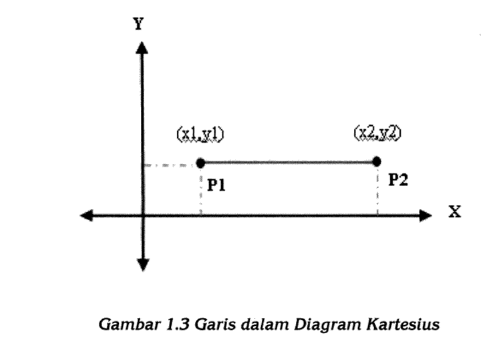
\includegraphics[width=1\textwidth]{figures/rahmi10.PNG}}
	\caption{penentuan garis pada kuadran katesius.}
	\label{rahmi10}
	\end{figure}

Dari dua buah titik diagram kartesius, bisa ditarik menjadi sebuah garis. Artinya pada sebuah garis memiliki titik awal


\section{Contoh Penerapan/Pemetaan Diagram Kartesius}
Tujuan digunakannya diagram kartesius adalah untuk melihat secara lebih terperinci mengenai atribut-atribut yang perlu untuk dilakukan perbaikan. 
Langkahlangkah sebelum memetakan data ke diagram kartesius ini, adalah terlebih dahulu dengan menentukan nilai rata-ratasetiap atribut yaitu X dan Y, 
dimana nilai perhitungannya telah kita peroleh dari perhitung yang dilakukan sebelumnya.
Adapun hasil pembagian setiap atribut pada setiap kuadaran ditampilkan pada gambar 2
\begin{figure}[ht]
	\centerline{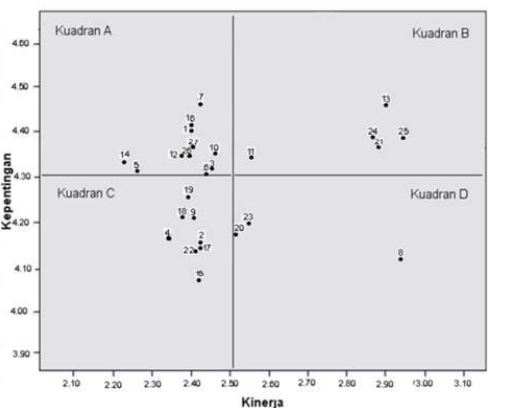
\includegraphics[width=1\textwidth]{figures/rahmi4.PNG}}
	\caption{.}
	\label{rahmi4}
	\end{figure}


Gambar 2. Diagram Kartesius
Setelah dilakukan perhitungan menggunakan diagram kartesius didapat hasil atribut-atribut yang harus diperbaiki adalah atribut yang berada pada kuadran A.
Adapun atribut yang harus diperbaiki pada kuadran A adalah :
Tabel 2 Hasil Perhitungan Diagram Kartesius pada Kuadran A	
\begin{figure}[ht]
	\centerline{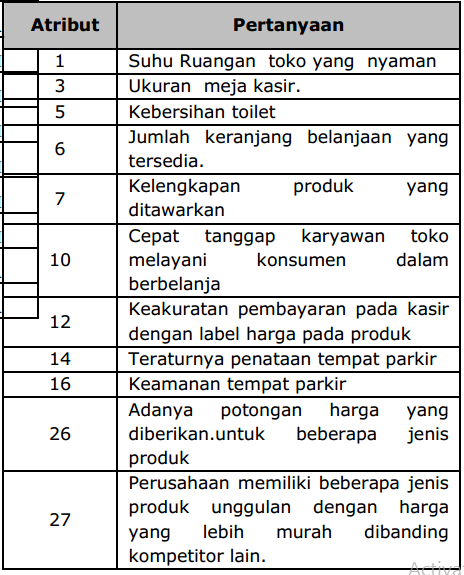
\includegraphics[width=1\textwidth]{figures/rahmi5.PNG}}
	\caption{.}
	\label{rahmi5}
	\end{figure}


Untuk atribut-atribut yang harus dipertahanan oleh pihak perusahaan setelah dilakukannya perhitungan menggunakan diagram kartesius adalah atribut-atribut
yang berada pada kuadran B, karena pada atribut yang berada pada kuadran B dianggap pelanggan sudah dapat memenuhi apa yang mereka inginkan. 
Adapun atribut yang harus dipertahankan dapat dilihat pada
Tabel 3.
Tabel 3. Hasil Perhitungan Diagram Kartesius
pada Kuadran B
\begin{figure}[ht]
	\centerline{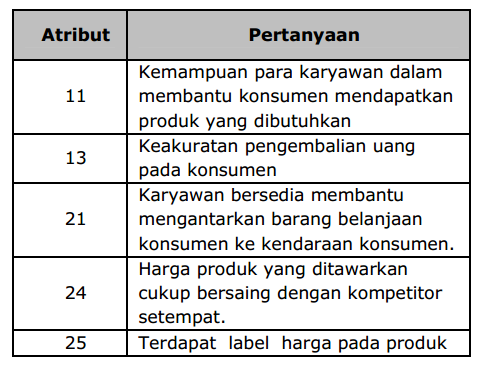
\includegraphics[width=1\textwidth]{figures/rahmi6.PNG}}
	\caption{.}
	\label{rahmi6}
	\end{figure}

Atribut yang memiliki penilaian yang rendah karena atribut-atribut ini kurang dianggap penting oleh pelanggan dan perusahaan juga tidak memberikan pelayanan atau perhatian khusus, 
atribut ini dianggap tidak memberikan dampak yang besar bagi perusahaan.
Adapun atribut-atribut yang berada pada kuadran C dapat dilihat pada Tabel 4.
Tabel 4. Hasil Perhitungan Diagram Kartesius pada kuadran C
\begin{figure}[ht]
	\centerline{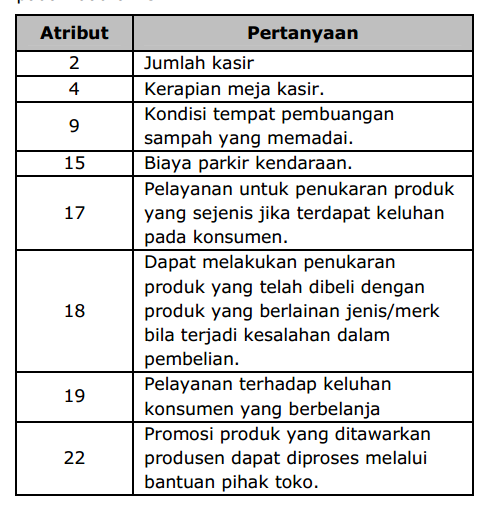
\includegraphics[width=1\textwidth]{figures/rahmi7.PNG}}
	\caption{.}
	\label{rahmi7}
	\end{figure}

Untuk atribut yang ada pada kuadran D adalah atribut yang tidak dianggap penting bagi pelanggan, namun pihak perusahaan memberikan pelayanan yang berlebihan 
sehingga atribut ini dianggap berlebihan.
Adapun atribut yang berada pada kuadran D dapat dilihat pada Tabel 5.
Tabel 5. Hasil Perhitungan Diagram Kartesius
pada Kuadran D	
\begin{figure}[ht]
	\centerline{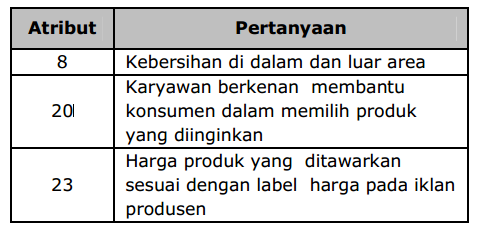
\includegraphics[width=1\textwidth]{figures/rahmi8.PNG}}
	\caption{.}
	\label{rahmi8}
	\end{figure}


Diagram Kartesius
Dari hasil perhitungan yang telah dilakukan sebelumnya, terdapat 17 atribut yang perlu dilakukan perbaikan (Action) danterdapat 10 atribut yang perlu mendapat
perhatian untuk dipertahankan oleh pihak perusahaan (Hold). Diagram Kartesius Dari hasil pemetaan yang dilakukan pada diagram kartesius dapat terlihat beberapa
atribut yang perlu untuk dilakukannya perbaikan dan atribut-atribut perlu untuk dipertahankan oleh pihak perusahaan yang terbagi kedalam kuadran-kuadran (A, B, C
dan D) sesuai dengan tingkat kesesuaian antara tingkat kepentingan pelanggan dan kinerja perusahaan, yaitu dengan tingkat kesesuaian sebesar 58.374.
Adapun hasil pemetaannya adalah sebagai berikut:
Kuadran A
Kuadran A adalah wilayah yang berisikan atribut-atribut yang dianggap penting oleh pelanggan, namun dalam kenyataannya atribut-atribut ini masih belum sesuai
dengan yang diharapkan oleh pelanggan. Dalam hal ini perusahaan perlu melakukan perbaikan sebaik mungkin untuk meningkatkan kepuasan pelanggan terhadap
atribut yang termasuk kedalam kuadran A. Dari diagram kartesius yang dibuat, diketahui bahwa atribut yang termasuk dalam kuadran A yaitu atribut 1, 3, 5, 6, 7,
10, 12, 14, 16, 26, 27.
Adapun beberapa hal yang sebaiknya perlu dilakukan guna perbaikan atau penyesuaian terhadap beberapa hal yang menjadi  prioritas diatas yang pertama antara lain
perlunya dilakukan penambahan alat pendingin ruangan untuk dapat menjaga suhu ruangan demi kenyamanan pelanggan,Penambahan ukuran meja kasir agarbarang-barang belanjaan yang telah dipilih
tidak merepotkan pelanggan ataupun kasir. Selain itu juga perlu dilakukannya perbaikan ataupun pembersihan ruangan toilet dan pendukung lainnya seperti ketersediaan air
sehingga pelanggan yang menggunakan akan merasa lebih nyaman, penambahan jumlah keranjang belanjaan yang disediakan perusahaan, Lebih melengkapi jenis-jenis
produk yang ditawarkan dengan mempertimbangkan tempat penyimpanan serta waktu-waktu tertentu seperti hari-hari besar nasional dan lain sebagainya,Memberikan pengarahan kepada para
karyawan mengenai pentingnya berinisiatif dalam melayani pelanggan yang membutuhkan bantuan tanpa harus dimintaitolong terlebih dahulu oleh pelanggan.
Dapat juga dilakukan penambahan papan informasi berupa lokasi produk yang tersedia untuk dapat mengurangi frekuensi terjadi atau timbulnya pertanyaan dari para
pelanggan mengenai produk yang akan mereka beli, perbaikan ataupun penyesuaian secara berkala antara labellabel harga yang tertera pada produk yang ditawarkan dengan perubahan-perubahan
harga yang terjadi, penataan tempat parkir yang dapat dilakukan dengan memberikan garis-garis pembatas kendaraan, ataupun dengan menambahkan tukang parkir untuk
dapat menanggulangi keamanan dan penataan tempat parkir kendaraan, penyusunan program-program promo secara berkala, seperti pemberian diskon denganjumlah pembelian tertentu ataupun dengan
memberikan voucer belanja dengan nilai tertentu untuk dapat lebih menarik pelanggan, dan sebaiknya perusahaan memiliki atau beberapa jenis produk tertentu
yang diunggulkan dengan harga yang lebih murah dibandingkan dengan kompetitor lainnya sebagai penarik.
Kuadran B
Kuadran B adalah daerah yang memuat atribut-atribut yang dianggap penting oleh pelanggan, dan atribut-atribut tersebut dianggap telah sesuai dengan keinginan
pelanggan sehingga tingkat kepuasan pelanggan relatif lebih tinggi, sehingga perlu untuk dipertahankan oleh pihak perusahaankarena sudah bisa memberikan pelayanan
sesuai dengan keinginan pelanggan sehingga konsumen merasa puas. Adapun atribut yang termasuk kedalam kuadran ini adalah:11, 13, 21, 24, 25.
Kuadran C
Kuadran C adalah Daerah yang berisikan atribut-atribut yang dianggap kurang penting oleh pelanggan dan pada kenyataannya kinerja pihak perusahaanpundinilai kurang memuaskan. Tetapi tidak
menutup kemungkinan Kuadran C pada waktu yang akan datang menjadi perhatian yang penting oleh pelanggan, sehingga perusahaan juga harus mempertimbangkan
hal tersebut. Adapun atribut yang termasuk kedalam kuadran ini adalah: 2, 4, 9, 15, 17, 18, 19, 22.
Kuadran D
Kuadran D adalah wilayah yang memuat atribut-atribut yang dianggap kurang penting oleh pelanggan dan kinerja yang dilakukan oleh pihak perusahaan dirasakan
terlalu tinggi atau berlebihan, sehingga perusahaan tidak perlu melakukan perbaikan. Adapun atribut yang termasuk kedalam kuadran ini adalah: 8, 20, 23.

\section{Pengertian Bidang atau Diagram Cartesius}

Dalam mempelajari materi himpunan, fungsi, dan persamaan garis lurus kita akan mengenal yang namanya bidang atau diagram Cartesius. Apa itu bidang atau diagram Cartesius?

Diagram Cartesius adalah sistem kordinat yang digunakan untuk meletakan titik pada penggambaran objek berdasarkan pemasukan nilai pada sumbu x dan nilai pada sumbu y dimana titik pertemuan ini nilai dari sumbu x dan sumbu y titik kordinat dibentuk. Jadi, diagram Cartesius digunakan untuk menentukan tiap titik dalam bidang dengan menggunakan dua bilangan yang biasa disebut koordinat x dan koordinat y dari titik tersebut. Di mana x disebut absis dan y disebut ordinat.

Titik-titik pada koordinat Cartesius merupakan pasangan titik pada sumbu-x dan sumbu-y (x, y). Perpotongan antara sumbu-x dan sumbu-y di titik 0 (nol) disebut pusat koordinat. Untuk bagian atas sumbu y bernilai positif, sedangkan pada bagian bawah sumbu y bernilai negatif. Begitu juga pada sebelah kanan sumbu x bernilai positif, sedangkan pada sebelah kiri sumbu x bernilai negatif. Untuk contohnya silahkan lihat gambar di bawah ini. 
\begin{figure}[ht]
	\centerline{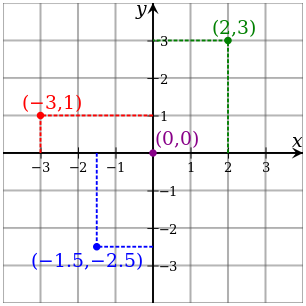
\includegraphics[width=1\textwidth]{figures/cau100.PNG}}
	\caption{penentuan garis/titik dalam diagram kartesius}
	\label{cau100}
	\end{figure}

Perhatikan diagram Cartesius pada gambar di atas. Warna ungu (violet) merupakan pusat koordinat yaitu titik (0,0) yang artinya sumbu x dan y bernilai nol. Untuk warna hijau, pada sumbu x bernilai 2 dan sumbu y bernilai 3 maka koordinat dalam bidang cartesius ditulis (2,3). Untuk warna merah, pada sumbu x bernilai  – 3 dan sumbu y bernilai 1 maka koordinat dalam bidang cartesius ditulis (– 3, 1). Sedangkan untuk warna biru, pada sumbu x bernilai  – 3 dan sumbu y bernilai 1 maka koordinat dalam bidang cartesius ditulis (–1.5 , –2.5).

Menurut wikipedia, istilah Cartesius digunakan untuk mengenang ahli matematika sekaligus filsuf dari Perancis bernama Descartes. Beliau memiliki peranan yang sangat besar dalam menggabungkan aljabar dan geometri (Cartesius adalah latinisasi untuk Descartes). Hasil kerjanya sangat berpengaruh dalam perkembangan geometri analitik, kalkulus, dan kartografi.




\chapter[Benua]
{Pengantar\\ benua}
% Kelompok Sejarah Benua dan Koordinat
% Agien Farhan S (1154012)
% Berlin Mitra Putra A (1154061)
% Indra Riksa Herlambang (1154051)
% Indra Saryoni Simanjuntak (1154115)
% Kindi Herdiansyah (1154048)

\section{Sejarah Benua}

\subsection{Benua pertama}
Mantel konveksi, proses yang mendorong lempeng tektonik adalah hasil dari aliran panas dari dalam bumi ke permukaan bumi \cite{suryasejarah}.Termasuk juga penciptaan lempeng tektonik di pegunungan bawah laut. Lempeng ini dihancurkan oleh subduksi di zona subduksi. Pada awal eon Arkean \ref{PetaAmerikaUtara} (sekitar 3 miliar tahun yang lalu) mantel itu jauh lebih panas mungkin sekitar 1600° C, sehingga proses konveksi terjadi lebih cepat.

Kerak bumi mulai terbentuk saat permukaan bumi mulai memadat, menghilangkan bekas-bekas pergeseran lempeng tektonik Hadean. Namun, diperkirakan kerak bumi memiliki komposisi Basalt seperti Kerak samudera .Potongan kerak benua besar yang pertama, muncul saat akhir masa Hadean, sekitar 4 miliar tahun yang lalu.  Kraton adalah bagian kecil yang tersisa dari benua pertama. Potongan-potongan yang terjadi pada akhir Hadean sampai awal Arkean membentuk inti lempengan yang tumbuh menjadi benua seperti sekarang.

Batuan tertua ditemukan di Laurentia, Kanada, yang berupa tonalit yang berumur sekitar 4 miliar tahun. Bebatuan ini menunjukkan jejak metamorfosis oleh suhu tinggi,  dan biji-bijian sedimen yang terkena erosi selama terbawa oleh air, yang menunjukkan terdapat sungai dan laut pada 4 miliar tahun yang lalu.

\begin{figure}[ht]
    \centerline{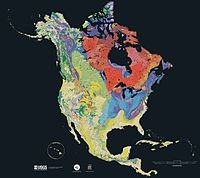
\includegraphics[width=1\textwidth]{figures/PetaAmerikaUtara.JPG}}
    \caption{Peta geologi Amerika Utara, kode warna menunjukan usia. Warna merah dan pink menunjukkan batuan dari masa eon Arkean.}
    \label{PetaAmerikaUtara}
    \end{figure}


\subsection{Benua raksasa pada masa Proterozoikum} 
Rekonstruksi pergerakan lempeng tektonik pada 250 juta tahun terakhir ( pada era Kenozoikum dan mesozoikum) dapat dilakukan dengan melihat kecocokan benua, anomali magnetik dasar laut, dan kutub paleomagnetik \cite{suryasejarah}. Para ahli tidak menemukan kerak samudera yang terbentuk sebelum waktu tersebut, sehingga rekonstruksi sebelum waktu tersebut sulit untuk dilakukan. Kutub paleomagnetik dilengkapi dengan bukti geologi seperti sabuk orogenik, yang menandai tepi lempeng kuno, dan distribusi flora dan fauna pada masa itu.

Sepanjang sejarah bumi, ada saat dimana benua bertabrakan dan membentuk benua raksasa, yang kemudian pecah menjadi benua baru. Sekitar 1000–830 juta tahun yang lalu, benua yang paling luas bersatu membentuk sebuah benua raksasa Rodinia. Sebelum Rodinia terbentuk, diperkirakan telah terbentuk terlebih dahulu Columbia atau Nuna pada awal sampai pertengahan masa Proterozoikum.

Setelah Rodinia pecah sekitar 800 juta tahun lalu, benua-benua tersebut kemungkinan telah membentuk benua raksasa lain yang berumur pendek yaitu , Pannotia \ref{BenuaRaksasaPannotia} pada 550 juta tahun lalu. Hipotetis benua raksasa mengacu pada Pannotia atau Vendia. Bukti yang memperkuat hipotesis tersebut adalah fase tabrakan benua yang diketahui sebagai orogeni Pan-Afrika, yang bergabung dengan benua Afrika , Amerika Selatan, Antartika dan Australia. Keberadaan Pannotia ditentukan oleh terjadinya retakan antara Gondwana (sebagian besar termasuk daratan di belahan bumi selatan, serta meliputi Semenanjung Arab dan anak benua India) dan Laurentia (kira-kira setara dengan Amerika Utara pada masa sekarang).Hal ini meyakinkan bahwa pada akhir masa eon Proterozoikum, sebagian besar benua bergabung dalam posisi di sekitar kutub selatan.

\begin{figure}[ht]
    \centerline{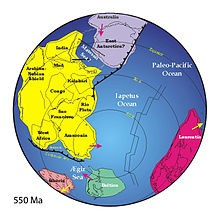
\includegraphics[width=1\textwidth]{figures/BenuaRaksasaPannotia.JPG}}
    \caption{Rekonstruksi benua raksasa Pannotia (warna kuning) pada 550 juta tahun lalu.}
    \label{BenuaRaksasaPannotia}
    \end{figure}


\subsection{Bukti Tersusunnya Benua Kuno}
Terdapat bukti dari para ahli yang digunakan untuk memperkirakan tersusunnya benua kuno.
Menurut Alfred Wegener(1880-1930), bahwa semua benua pernah bersatu kemudian berpecah menjadi sekarang ini dan benua yang bersatu itu dinamakan Pagaea (Benua Besar)\cite{hallam1975alfred}. Kemudian para ahli meneliti tentang benua dan membuat spekulasi-spekulasi teoritis yaitu melihat pada peta bahwa benua saling melengkapi dilihat dari garis pantai yang saling melengkapi seperti bagian puzzle. Kemudian meneliti fosil, bukti lain dari kehidupan lampau yaitu Mesosaurus. Mesosaurus adalah reptilia purba yang hanya hidup di air tawar dan ternyata hanya ada dua kawasan didunia yang memiliki fosil Mesosaurus ini yaitu Pantai Timur Amerika Selatan dan Pantai Barat Afrika. Kesimpulannya, fosil yang sama telah ditemukan di dalam batuan di kedua sisi lautan. Kemudian bukti korelasi batuan dan pegunungan telah ditemui di kedua belah sisi lautan. Yaitu meneliti banjaran pegunungan di Timur Laut Amerika Serikat dan banjaran pegunungan di Utara Eropa. Keduanya sangat sepadan atau keduanya tersusun daripada jenis batuan yang sama. Kemudian bukti data iklim masa lalu, terbukti pada Glacial Striations atau terdapat bentuk goresan pada batuan dan ini dapat dilihat dari hutan hujan tropika Amerika Selatan dan Afrika saat ini terdapat goresan glasier. Kesimpulannya adalah arang batu telah ditemukan di kawasan sejuk dan bukti glasier telah ditemui di kawasan panas berarti sebelumnya ada kemungkinan benua bersatu.

\section{Sejarah Koordinat}
Menurut ahli sejarah yang bernama Heroditus (450 M) menyatakan bahwa geometri berasal dari Mesir. Rane Discartes seorang matematikawan, yang lahir di sebuah Desa La Haye Prancis pada tahun 1596, adalah orang yang memiliki ketertarikan di bidang geometri. Rane Descrates telah menemukan sebuah metode untuk menyajikan sebuah titik sebagai bilangan berpasangan pada sebuah bidang datar. Bilangan-bilangan tersebut terletak pada dua garis yang saling tegak lurus antara satu dengan lainnya dan berpotongan di sebuah titik (0,0) dinamakan Origin , dan biasanya disimbolkan dengan huruf kapital O (0,0).
Bidang tersebut dinamakan bidang KOORDINAT atau yang lebih dikenal dengan bidang KARTESIUS.

\section{Sistem Koordinat}
Sistem koordinat dimaksudkan untuk memberikan peng-alamat-an terhadap setiap lokasi di permukaan bumi. Peng-alamatan dengan sistem kordinat didasarkan atas jarak timur-barat dan utara-selatan suatu tempat dari suatu titik pangkal tertentu. Jarak diukur dalam satuan derajat sudut yang dibentuk dari dari titik pangkal ke posisi tersebut melalui pusat bumi. Sedangkan titik pangkal ditetapkan berada di
perpotongan belahan utara-selatan bumi (garis katulistiwa) dengan garis yang membelah bumi timur- barat\cite{zuhdi2012sistem}.

Koordinat diambil untuk menjadi bilangan riil dalam matematika dasar, tetapi mungkin bilangan kompleks atau elemen-elemen dari sistem yang lebih abstrak. Penggunaan sistem koordinat memungkinkan masalah dalam angka untuk diterjemahkan ke dalam masalah-masalah tentang geometri dan juga sebaliknya.

\subsection{Sistem Koordinat Dua Dimensi}
\subsubsection{Sistem Koordinat Kartesius}
Koordinat Cartesius bukan merupakan satu-satunya jalan untuk menunjukkan kedudukan suatu titik pada bidang. Karena bentuk geometris di alam tidak selalu berupa kotak-kotak atau persegi panjang, namun adakalanya berbentuk lingkaran\cite{mufidah2015solusi}.Sistem koordinat Kartesius pada dua dimensi umumnya didefinisikan dengan dua buah sumbu yang saling tegak lurus antara satu dengan yang lainnya, yang keduanya terletak pada satu bidang (bidang xy). Sumbu horizontal(x), dan sumbu vertikal(y). Lalu, pada sistem koordinat tiga dimensi, ditambahkan sumbu yang lain yang sering diberi label z. Sumbu-sumbu tersebut ortogonal antar satu dengan yang lainnya. Titik pertemuan antara kedua sumbu, titik asal, pada umumnya diberi label 0. Setiap sumbu juga memiliki besaran panjang unit, dan setiap panjang tersebut diberi tanda dan membentuk semacam grid. Untuk mendeskripsikan suatu titik tertentu pada sistem koordinat dua dimensi, nilai absis(x), lalu diikuti dengan nilai ordinat(y). Dengan demikian, format yang dipakai selalu (x dan y) dan urutannya tidak dibalik-balik.

Gambar \ref{koordinat} Tanda panah yang ada pada sumbu berarti panjang sumbunya tak terhingga pada arah panah tersebut.

\begin{figure}[ht]
    \centerline{\includegraphics[width=1\textwidth]{figures/koordinat.JPG}}
    \caption{Keempat kuadran sistem koordinat Kartesius}
    \label{koordinat}
    \end{figure}

Pilihan huruf-huruf didasari oleh konvensi, yaitu huruf-huruf yang dekat akhir(x dan y) yang digunakan untuk menandakan variabel dengan nilai yang tidak diketahui, sedangkan huruf-huruf yang lebih dekat awal digunakan untuk menandakan nilai yang diketahui. Karena kedua sumbu saling bertegak lurus satu sama lain, bidang xy terbagi menjadi empat bagian yang disebut dengan kuadran, yang pada Gambar 3 ditandai dengan angka I, II, III, dan IV. Menurut konvensi yang berlaku, keempat kuadran tersebut diurutkan mulai dari yang kanan atas (kuadran I), melingkar melawan arah jarum jam (lihat Gambar 3). Pada kuadran I, kedua koordinat (x,y) bernilai positif. Pada kuadran II, koordinat x bernilai negatif dan koordinat y bernilai positif. Pada kuadran III, kedua koordinat mempunyai nilai negatif, dan pada kuadran IV, koordinat x bernilai positif dan y bernilai negatif. (lihat gambar \ref{contoh} dibawah ini).

\begin{figure}[ht]
    \centerline{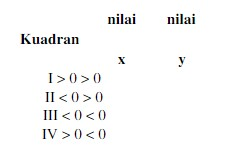
\includegraphics[width=1\textwidth]{figures/contoh.JPG}}
    \caption{Nilai x dan y pada Kuadran I,II,III,IV}
    \label{contoh}
    \end{figure}

\subsubsection{Sistem Koordinat Polar}
Pada sistem koordinat polar, sepasang koordinat polar suatu titik ditulis dengan (𝑟,𝜃)\cite{mufidah2015solusi}.Konsep dari sudut dan radius sudah diterapkan oleh orang-orang pada zaman dahulu se-abad sebelum masehi. Para astronom yunani dan astrologhipparcuhus (190-120 BCE) menemukan sebuah tabel dari fungsi dawai yang memberikan panjang dawai dari setiap sudut dan terdapat referensi dari penggunaan koordinat polar untuk mengetahui posisi bintang.

Sejak abad ke-8 yang lalu, astronom mengembangkan cara untuk mengira-ngira dan menghitung arah dari mekah, kaabah- beserta jaraknya-dari seluruh lokasi dari bumi. Penghitungan penting yaitu penggantian dari koordinat polar ekuatorial dari mekkah kedalam bentuk koordinat polar hampir sama pada sistem yang merupakan pusat dari lingkaran besar melewati daerah yang dilewati dan kutub bumi, serta sudut polar yaitu garis yang melewati daerah tersebut dan titik antipodal.

Dalam Method of fluxion (tertulis 16711) Sir Isaac Newton menentukan hubungan antara koordinat polar, yang kemudian ia sebut dengan “ tujuh cara untuk spiral, dan sembilan sistem koordinat. 

\section{Geometri Koordinat}
 Pembelajaran subtajuk-subtajuk Geometri Koordinat, iaitu jarak antara dua titik, pembahagian tembereng garis, luas poligon, persamaan garis lurus, garis lurus selari dan garis lurus serenjang, persamaan lokus yang melibatkan jarak antara dua titik dan menentukan hubungan antara pencapaian responden dalam topik pelajaran\cite{shong2013analisis}.
 
 \subsection{Sketsa Grafik Garis}
 Sketsa grafik garis merupakan salah satu materi yang membahas mengenai penggambaran grafik garis lurus pada bidang kartesius berdasarkan persamaan yang diberikan. Materi ini mirip dengan metode penggambaran garis yang ada atau diajarkan pada aljabar. Maka jika sudah menguasai materi aljabar, sketsa grafik garis bukan masalah untuk dipelajari. Dalam menggambar grafik garis lurus, pertama harus melakukan pencarian pada nilai x dan y pada bidang kartesius dari persamaan yang sudah ada. Setelah nilai x dan y pada bidang kartesius telah di-temukan tentu bisa menentukan titiknya dan langsung menggambar garis tersebut.
 
 \subsection{Persamaan Garis Lurus}
 Persamaan garis lurus dapat di-definisikan sebagai perbandingan selisih nilai x dan y yang sudah melangkahi 2 titik pada garis. 
 Persamaan garis lurus terdapat satu komponen Gradien yaitu kecenderungan sebuah garis, gradien biasa dilambangkan dengan huruf m.
 Dalam materi persamaan garis lurus terdapat materi pokok seperti menentukan \"gradien" garis lurus, \"kedudukan" garis lurus,
 \"persamaan" garis melalui satu titik merupakan gradien, dan \"persamaan" garis melalui dua titik.
 
 \subsection{Pesamaan Lingkaran}
 Persamaan lingkaran adalah persamaan titik koordinat yang membentuk sebuah lingkaran pada bidang kartesius. Pada konsep ini jari lingkaran yang telah terbentuk adalah jarak dari himpunan titik koordinat ke titik pusat atau sebaliknya.Pada persamaan lingkaran yang dapat dipelajari seperti lingkaran yang memiliki pusat (0,0), lingkaran yang memiliki pusat (a,b).
 
 \subsection{Program Linear}
 Program linear adalah metode matematika yang digunakan untuk menyelesaikan soal-soal yang memiliki batas persamaan linear. Secara umum program linear terbagi atas 2 bagian yaitu fungsi kendala dan fungsi objektif. Penyelesaian program linear model matematika adalah suatu metode penerjemahan permasalahan ke dalam bentuk matematika, sehingga soal tersebut bisa diselesaikan secara matematis.
 
 \subsection{Pembelajaran Geometri Koordinat}
 Geometri Koordinat merupakan materi yang memberika pengujian ketrampilan dalam geometri dan aljabar.
 Jika sudah menguasai materi geometri dan aljabar maka bisa dinyatakan geometri koordinat tidak lagi membuat sulit untuk dipelajari.


\chapter[Sejarah Bumi]
{Pengantar\\ Sejarah Bumi}
% Nama Kelompok : Kelompok 4
% Akbar Pambudi Utomo (1154094) 
% Andi Nurfadilah Ali (1154041)
% Andi Wadi Afryandika (1154113)
% Hanna Theresia Siregar (1154009)
% Julham Ramadhana (1154069)
% Pebridayanti Hasibuan (1154118)

\section{Sejarah Bumi}
Bumi merupakan planet atau rumah kita dalam kedudukan di tata surya. peradaban kuno percaya bahwa bumi itu datar, dengan langit berputar-putar sekali sehari. secara umum yang diyakini bahwa kehidupan di Bumi dimulai di Bumi itu sendiri, beberapa waktu setelah terbentuknya planet antara 4000-5000 juta tahun yang lalu. namun ada yang berpendapat bahwa kehidupan diluar bumi itu ada, tetap kita tidak memiliki bukti pasti tentang kehidupan di tempat lain. yang perlu kita ketahui bumi berada pada galaksi bimasakti dimana terdapat matahari sebagai sistem bintang.
Dalam Geologi sendiri atau biasa disebut sebagai ilmu pengetahuan tentang Kebumian yang mempelajari segala sesuatu mengenai planet Bumi beserta isinya yang pernah ada. Dalam Geologi juga akan dibahas tentang sifat-sifat dan bahan- bahan yang membentuk bumi itu apa, serta struktur dan proses-proses yang bekerja baik didalam maupun dibagian teratas permukaan bumi, kedudukannya di Alam Semesta hingga sekarang. Geologi merupakan ilmu pengetahuan yang komplek, mempunyai pembahasan materi yang beraneka ragam namun juga merupakan ilmu pengetahuan yang enak dipelajari. Sebagai landasan prinsip untuk dapat mempelajari ilmu geologi adalah bahwasanya kita harus menganggap bumi ini sebagai suatu benda yang secara dinamis berubah sepanjang masa, setiap saat dan setiap detik. 
Pemikiran geologi modern dikenalkan oleh Huttonian revolution mengemukakan pemikiran-pemikirannya sebagai berikut:
1. Bahwasanya proeses-proses alam yang sekarang ini menyebabkan perubahan pada permukaan bumi, juga bekerja sepanjang umur dari bumi ini. 
2. Ia juga mengamati bahwa proses-proses tersebut yang walaupun bekerja sangat lambat, tetapi pada akhirnya mampu menyebabkan terjadinya perubahan-perubahan yang sangat besar pada bumi. 
3. Bahwa bumi ini sangat dinamis, yang berarti mengalami perubahan-perubahan yang terus-menerus mengikuti suatu pola daur (siklus) yang berulang-ulang.
Bumi sendiri berada di kawasan dimana terjadinya tumpang tindih antara litosfer (daratan) bagian padat dari bumi, hidrosfer (perairan), dan atmosfer (udara) yang menyelubungi bumi dengan zarah-zarah dan benda-benda yang mengisinya.
Dalam sejarah terbentuknya bumi sewaktu SMA kita pernah mempelajari teori-teori terbentuknya bumi dalam pelajaran geografi.\cite{wetherill1990formation}

\subsection{Teori-teori terbentuknya Bumi}
\subsubsection{1.Teori Kabut Kant-Laplace}
\begin{figure} [ht]
	\centerline{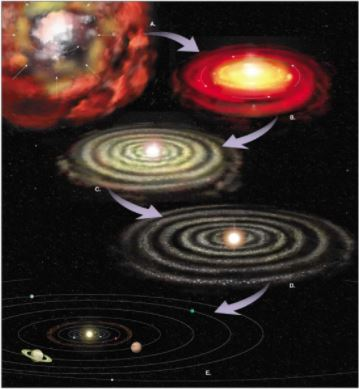
\includegraphics[width=1\textwidth]{figures/teorikabutnebula.JPG}}
	\caption{Gambar Teori Nebula}
	\label{teorikabutnebula}
	\end{figure}
	Pada Gambar berikut \ref{teorikabutnebula} adalah gambar dari Teori Kabut Nebula.
Teori ini dikenal dengan teori kabut (nebula) yang dikemukakan oleh Immanuel Kant (1755) dan Pierre de Laplace (1796). dalam teori ini dikemukakan bahwa di jagat raya terdapat gas yang kemudian berkumpul menjadi kabut(nebula). gaya tarik-menarik antargas ini membentuk kumpulan kabut yang sangat besar dan berputas semakin cepat sehingga materi kabut bagian khatulistiwa terlempar memisah dan memadat(karena pendinginan), bagian yang terlempar inilah yang kemudian menjadi sebuah planet dalam tatasurya. Bumi baru terus bertumbuh sampai suhu interiornya cukup panas untuk melelehkan logam siderofil. Dengan massa jenis yang lebih tinggi dari silikat, akhirnya logam ini tenggelam. Proses ini terjadi 10 juta tahun setelah Bumi mulai terbentuk, dan menghasilkan struktur Bumi yang berlapis-lapis dan mengakibatkan terbentuknya medan magnet. J. A. Jacobs merupakan orang pertama yang menunjukkan bahwa inti dalam—bagian dalam yang padat berbeda dari inti luar yang padat—membeku dan mengembang keluar inti luar yang cair dikarenakan bagian dalam bumi yang makin mendingin (sekitar 100° C per miliar tahun. Ekstrapolasi dari pengamatan ini memperkirakan bahwa inti terbentuk pada masa 2–4 miliar tahun yang lalu. Jika ini benar maka berarti bahwa inti bumi bukanlah fitur primordial yang berasal selama pembentukan planet.

\subsubsection{2.Teori Planetesimal}
\begin{figure} [ht]
	\centerline{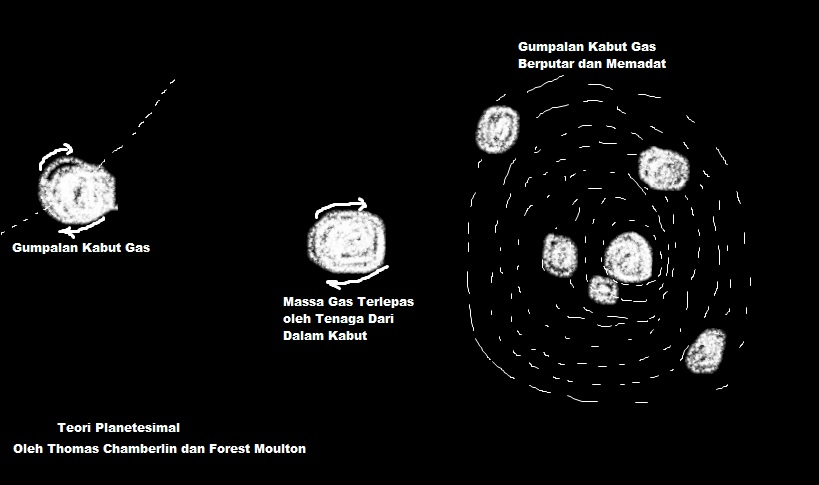
\includegraphics[width=1\textwidth]{figures/teoriplanetesimal.JPG}}
	\caption{Gambar Teori Planetesimal}
	\label{teoriplanetesimal}
	\end{figure}
	Pada Gambar berikut \ref{teoriplanetesimal} adalah gambar dari Teori Planetesimal.
seabad kemudian sesudah teori kabut tersebut muncul teori Planetesimal yang dikemukakan oleh Chamberlin dan Moulton. Teori ini mengungkapkan bahwa pada mulanya telah terdapat Matahari asal. pada suatu ketika, matahari asal ini didedakti sebuah bintang besar yang menyebabkan terjadinya penarikan pada bagian matahari. Akibat tenaga tarik menarik tadi, terjadilah ledakan yang dasyat. Gas yang meledak ini keluar dari atmosfer matahari, kemudian mengembun dan membeku sebagai benda-benda yang padat(disebut planetesimal). Planetesimal ini dalam perkembangannya menjadi planet-planet, dan salah satunya planet bumi kita.

\subsubsection{3.Teori Pasang Surut Gas}
\begin{figure} [ht]
	\centerline{\includegraphics[width=1\textwidth]{figures/teoripasangsurut.JPG}}
	\caption{Gambar Pasang Surut}
	\label{teoripasangsurut}
	\end{figure}
	Pada Gambar berikut \ref{teoripasangsurut} adalah gambar dari Teori Pasang Surut.
Teori ini dikemukakan oleh Jeans dan Jeffreys, yakni bahwa sebuah bintang besar mendekati matahari dalam jarak pendek, sehingga menyebabkan terjadinya pasang surut pada tubuh matahari. dalam lidah yang panas ini terjadi perapatan gas-gas dan akhirnya kolom-kolom ini akan pecah, lalu berpisah menjadi benda-benda tersendiri yaitu planet-planet. bintang besar yang menyebabkan penarikan pad abagian-bagian tubuh matahari tadi melanjutkan perjalanan di jagat raya, sehingga lambat laun akan hilang pengaruhnya terhadapt planet-planet yang terbentuk tadi, lalu planet-planet itu akan mengelilingi matahari dan mengalami proses pendinginan, proses pendinginan berjalan lambat pada planet besar seperti yupiter dan saturnus, sedangkan planet kecil seperti bumi mengalami proses pendinginan yang relatif lebih cepat.

\subsubsection{4. Teori Bintang Kembar}
\begin{figure} [ht]
	\centerline{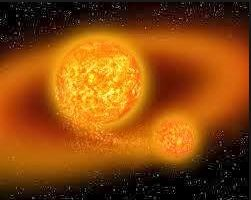
\includegraphics[width=1\textwidth]{figures/teoribintangkembar.JPG}}
	\caption{Gambar Teori Bintang Kembar}
	\label{teoribintangkembar}
	\end{figure}
	Pada Gambar berikut \ref{teoribintangkembar} adalah gambar dari Teori Bintang Kembar.
Teori ini dikemukakan oleh seorang ahli astronomi R. A. Lyttleton. Menurut teori ini, galaksi berasal dari kombinasi bintang kembar. Salah satu bintang meledak sehingga banyak materi yang terlempar. Karena bintang yang tidak meledak mempunyai gaya gravitasi yang masih kuat, maka sebaran pecahan ledakan bintang tersebut mengelilingi bintang yang tidak meledak. Bintang yang tidak meledak itu adalah matahari, sedangkan pecahan bintang yang lain itu adalah planet-planet yang mengelilinginya.

\subsubsection{5. Teori Dentuman Besar (Big Bang Teory)}
\begin{figure} [ht]
	\centerline{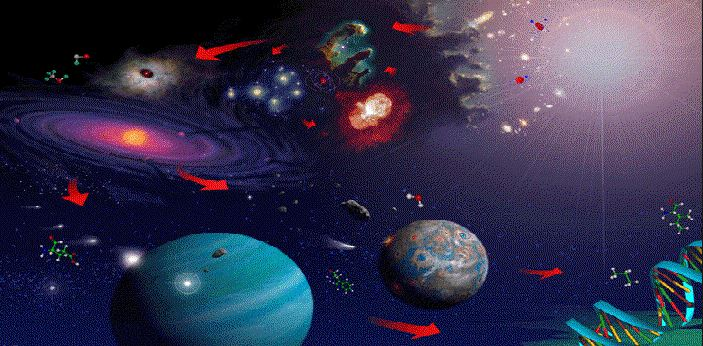
\includegraphics[width=1\textwidth]{figures/teoribigbang.JPG}}
	\caption{teoribigbang}
	\label{teoribigbang}
	\end{figure}
	Pada Gambar berikut \ref{teoribigbang} adalah gambar dari Teori Dentuman Besar(BigBang).
Pada Teori ini berdasarkan dari asumsi adanya massa yang sangat besar dan mempunyai massa jenis sangat besar. Adanya reaksi inti menyebabkan massa tersebut meledak hebat. Massa tersebut kemudian mengembang dengan sifat sangat cepat menjauhi pusat ledakan, karena danya gravitasi, maka bintang yang paling kuat gravitasinya akan menjadi pusatnya.
Dari berbagai teori, teori ini yang paling banyak didukung oleh para ilmuwan.

\section{Pendapat Tentang Sejarah Bumi}
Bumi terbentuk sekitar 4,54 miliar (4,54×109) tahun yang lalu melalui akresi dari nebula matahari. Pelepasan gas vulkanik diduga menciptakan atmosfer tua yang nyaris tidak beroksigen dan beracun bagi manusia dan sebagian besar makhluk hidup masa kini. Sebagian besar permukaan Bumi meleleh karena vulkanisme ekstrem dan sering bertabrakan dengan benda angkasa lain. Sebuah tabrakan besar diduga menyebabkan kemiringan sumbu Bumi dan menghasilkan Bulan. Seiring waktu, Bumi mendingin dan membentuk kerak padat dan memungkinkan cairan tercipta di permukaannya. Bentuk kehidupan pertama muncul antara 2,8 dan 2,5 miliar tahun yang lalu. Kehidupan fotosintesis muncul sekitar 2 miliar tahun yang lalu, nan memperkaya oksigen di atmosfer. Sebagian besar makhluk hidup masih berukuran kecil dan mikroskopis, sampai akhirnya makhluk hidup multiseluler kompleks mulai lahir sekitar 580 juta tahun yang lalu. Pada periode Kambrium, Bumi mengalami diversifikasi filum besar-besaran yang sangat cepat. Perubahan biologis dan geologis terus terjadi di planet ini sejak terbentuk. Organisme terus berevolusi, berubah menjadi bentuk baru atau punah seiring perubahan Bumi. Proses tektonik lempeng memainkan peran penting dalam pembentukan lautan dan benua di Bumi, termasuk kehidupan di dalamnya. Biosfer memiliki dampak besar terhadap atmosfer dan kondisi abiotik lainnya di planet ini, seperti pembentukan lapisan ozon, proliferasi oksigen, dan penciptaan tanah.Dalam sebuah artikel dari zuhdi2012sistem yang menyebutkan bahwa Bumi merupakan salah satu planet yang berada dalam tata surya yang diduga terbentuk dari pecahan-pecahan bintan pada jutaan tahun yang lalu, dan kemudian terperangkapa pada gravitasi matahari sehinggan akan selalu mengelilingi matahari. Menurut Hukum Newton kenapa planet dapat bertahan dalam pergerakan keliling atau biasa disebut revolusi dikarenakan planet melakukan gerak melingkar yang menimbulkan gaya sentifugal yang besarnya  dengan gaya gravitasi namun berlawanan arah. Gaya gravitasi ini sendiri akan berkurang sesuai dengan semakin jauhnya jarak planet dari matahari, sedangkan gaya sentrifugal  akan tergantung pada kecepatan gerak melingkar planet. Semakin cepat gerakan tersebut maka akan semakin besar daya sentifugal. Bila secara kebetulan kedua gaya ini memiliki kecepatan yang sama besar, maka planet akan terjebak mengelilingi matahari. Pada saat tata surya terbentuk diperkirakan terdapat jutaan planet. Akan tetapi sebagian terjatuh ke matahari atau terlempar lepas dari pengaruh matahari. Selain berkeliling, planet juga akan bergerak memutari pororsnya (rotasi). Gerak rotasi ini sendiri berlangsung dalan waktu lama sehingga membuat planet berbentuk seperti bola. Pada masa lalu, planet planet bukanlah sebuah benda padat, melainkan berupa magma atau berupa cairan batu. Bagian padat pada planet terbentuk selama proses pendinginan dan terjadi pada bagian kulit terluar dari planet tersebut. Bentuk Bumi sendiri yang dikatakan berbentuk bola tidakalah sempurna. Gerak Rotasi telah mengubah bentuk bumi menjadi agak cepat terhadap kedua kutubnya.\cite{zuhdi2012sistem}


Sejarah pembentukan Bumi yang dipelajari dalam materi pelajaran Geografi cenderung memiliki sifat abstrak yang akan lebih mudah dimengerti, jika memakai media yang cocok. Salah satu Inovasi pembelajaran yang tepat untuk dilakukan adalah menggunakan kartu indeks dan media film. Media seperti kartu indeks yang dipergunakan sebaga salah satu upaya yang memudahkan peserta didik agar mengingat konsep-konsep materi yang sedang dipelajari sedangkan media film sendiri merupakan media visual yang akan menjelaskan dengan lebih konkrit tentang fenomena bumi. Dalam sebuah artikel dari @article{widiyati2011meningkatkan menyebutkan bahwa Pmebentukan Bumi dengan kategori Continental Drift Theory atau biasa disebut dengan teori pengapungan benua yang dikemukan oleh Alfred Wegener pada tahun 1912 mengemukakan bahwa sampai sekitar 255 juta tahun lalu, di bumi baru ada satu benua dan samudera yang sangat luas. Benua raksasa ini sendiri dinamakan pangea, sedangkan kawasan samudera yang mengapitnya itu mengalami retakan-retakan dan pecah. Sekitar 135 juta tahun lalu, benua raksasa tersebut pecah menjadi dua, yaitu pecahan benua di sebelah utara yang dinamakan Lauransia dan dibagian selatan dinamakan gondwana.
\cite{widiyati2011meningkatkan}


\chapter[Garis Khatulistiwa]
{Pengantar\\ Garis Khatulistiwa}
   
								   
								   
												           Sejarah Garis Khatulistiwa Dan Prime Meridien
%Kelompok 4
% Eka Pratama Putra (1154023)
% Deni Braja Astrajingga (1154066)
% Luqman Nurfajri (1154054)
% Shinta Amelia (1154047)
% Yoshi Ricowandi Nababan (1154125)

														   
\section {Pendahuluan}

\subsection{pengertian garis khatulistiwa}	

	Dalam sebuah artikel dari Muhammad Adieb yang menyebutkan bahwa garis khatulistiwa merupakan garis lintang dari 0 derajat sampai dengan 90 derajat 
di kutub bumi. Jadi, nilai lintang berkisar antara 0° sampai dengan 90°. Di sebelah selatan garis khatulistiwa disebut lintang selatan (LS) dengan 
tanda negatif (-) dan di sebelah utara garis khatulistiwa disebut lintang utara (LU) yang diberi tanda positif (+). \cite {adieb2014studi}.

\subsection{pengertian prime meridian}
	
	Dalam sebuah artikel dari Mohd Zuhdi yang menyebutkan bahwa Prime meridian atau meridian Greenwich adalah nilai koordinat garis bujur dimulai dari 
bujur 0 derajat yaitu di Greenwich, kemudian membesar ke arah timur dan barat sampai bertemu kembali di Garis batas internasional yaitu terletak 
di Selat Bering dengan nilai 180 derajat. \cite {zuhdi2012sistem}.

	Dalam sebuah artikel lain oleh Andi Sunyoto yang menyebutkan bahwa Prime meridian adalah sebuah garis virtual yang melewati sebuah kota 
bernama Greenwich di Inggris. \cite{sunyoto2009api}.

\section {Isi}

\subsection{sistem koordinat bumi}
	
	Menurut sebuah artikel dari Mohd Zuhdi yang menyebutkan bahwa dalam sebuah artikel dari Mohd Zuhdi yang menyebutkan bahwa sistem koordinat dimaksudkan 
untuk memberikan pengalamatan terhadap setiap lokasi di permukaan bumi. pengalamatan dengan sistem koordinat didasarkan atas jarak timur sampai dengan barat 
dan utara sampai dengan selatan suatu tempat dari suatu titik pangkal tertentu. jarak diukur dalam satuan derajat dengan sudut yang dibentuk dari titik 
pangkal ditetapkan yang berada di perpotongan belahan utara sampai dengan selatan bumi (garis khatulistiwa) dengan garis yang membelah bumi bagian timur sampai 
dengan barat melewati kota GreenWhich di Inggris.

	
\begin{figure}[ht]
\centerline{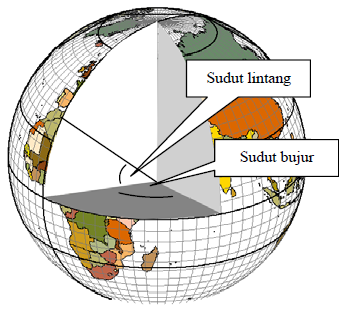
\includegraphics[width=1\textwidth]{figures/garis_lintang_dan_bujur.PNG}}
\caption{menjelaskan tentang sudut lintang dan bujur pada bumi.}
\label{garis_lintang_dan_bujur}
\end{figure}

Pada gambar \ref{garis_lintang_dan_bujur} menjelaskan tentang sudut lintang dan bujur pada bumi.

	Posisi suatu tempat di alamatkan dengan nilai koordinat garis bujur (longitude) dan lintang (latitude) yang melalui tempat itu. Garis bujur (longitude), 
biasanya juga disebut garis meridian, yaitu merupakan garis lurus yang menyambungkan dari kutub utara sampai selatan bumi. Nilai koordinat garis bujur ini dimulai dari
bujur 0 derajat yaitu di Greenwich, kemudian membesar ke arah timur dan barat sampai bertemu kembali di Garis batas internasional yaitu terletak 
di Selat Bering dengan nilai 180 derajat. Garis bujur 0 derajat sering disebut prime meridien atau meridian Greenwich. Garis bujur ke arah barat diberi 
nilai negatif dan disebut bujur barat (west longitude) serta disingkat BB. Sedangkan garis bujur yang ke arah timur diberi nilai positif 
dan disebut bujur timur (east longitude) disingkat BT. Nilai koordinatnya didasarkan atas besarnya sudut yang terbentuk dari bujur 0 ke garis bujur tersebut
 melalui pusat bumi.

	Adapun nilai koordinat lintang dimulai dari garis lingkaran khatulistiwa yang diberi nilai 0 derajat. Selanjutnya garis-garis lintang yang lain berupa 
lingkaran-lingkaran paralel (sejajar) khatulistiwa berada di sebelah utara dan selatan khatulistiwa. Lingkaran paralel di selatan disebut garis lintang selatan (LS)
dan diberi nilai negatif, sedangkan lingkaran paralel di utara  diberi  nilai positif dan disebut garis lintang utara (LU). Nilai maksimum koordinat 
garis lintang adalah 90 derajat yaitu terletak di kutub-kutub bumi.

	Lingkaran paralel yang merupakan representasi garis lintang ini semakin mengecil ukurannya dengan semakin jauh dari khatulistiwa. Sehingga jarak 1 derajat 
timur sampai barat hanya beberapa meter saja. Itu sebabnya grid yang dibuat dari garis lintang dan garis bujur, tampaak berupa bujur sangkar di khaatulistiwa 
dan berubah menjadi persegi panjang di daerah dekat kutub. \cite {zuhdi2012sistem}.

\subsection (pemanfaatan prime meridian)

	Meridian Utama atau Prime Meridien digunakan untuk menentukan waktu di dunia, metode penentuannya akan dijelaskan sebagai berikut

\subsubsection(sistem penentuan waktu dunia)
	
	Menurut sebuah artikel dari Misbah Khusurur dan Jaenal Arifin yang menyebutkan bahwa Waktu Universal (bahasa Inggris Universal Time, disingkat UT)
adalah satu ukuran waktu yang didasari oleh rotasi bumi. Satuan ini adalah model perhitungan modern dari GMT (Greenwich Mean Time), yaitu mean waktu matahari 
di meridian di Greenwich, Inggris, yang biasanya dianggap sebagai bujur geografis 0 derajat GMT ini merupakan waktu 4 pertengahan yang yang di dasari oleh 
garis bujur yang melalui Greenwhich (BB/BT 0°) dan digunakan sebagai standar waktu Dunia Internasional.
	
	Sebelum diperkenalkannya standar waktu, setiap kota menyetel waktunya sesuai dengan posisi matahari di tempat masing-masing. Sistem ini bekerja 
dengan baik sampai diperkenalkannya transportasi kereta api untuk berpergian dengan cepat. akan tetapi, memerlukan seseorang untuk terus-menerus mencocokan 
jamnya dengan waktu lokal yang berbeda-beda dari satu kota ke kota lain. Standar waktu, dimana semua jam di dalam satu daerah menggunakan waktu yang sama, 
dibuat untuk memecahkan masalah perbedaan waktu seperti dalam perjalanan kereta api di atas.

	Standar waktu ini membagi bumi kedalam beberapa bagian ”zona waktu”, masing-masing bagiannya mencakupi dengan paling sedikit 15 derajat. Semua jam di dalam
zona waktu ini disetel sama dengan jam lainnya, tapi berbeda sebanyak satu jam dari jam-jam di zona waktu yang bertetanggaan. 
Waktu lokal di Royal Greenwich Observatory di Greenwich, Inggris, dipilih sebagai standard waktu dunia setelah terjadi 
Konferensi Meridian Internasional tahun 1884, yang memicu penyebaran pemakaian Greenwich Mean Time untuk menyetel jam di dalam suatu daerah. 
Lokasi ini dipilih sampai tahun 1884, 66 % dari semua peta dan tabel menggunakan greenwhich sebagai meridian utama (prime meridian).

\begin{figure}[ht]
\centerline{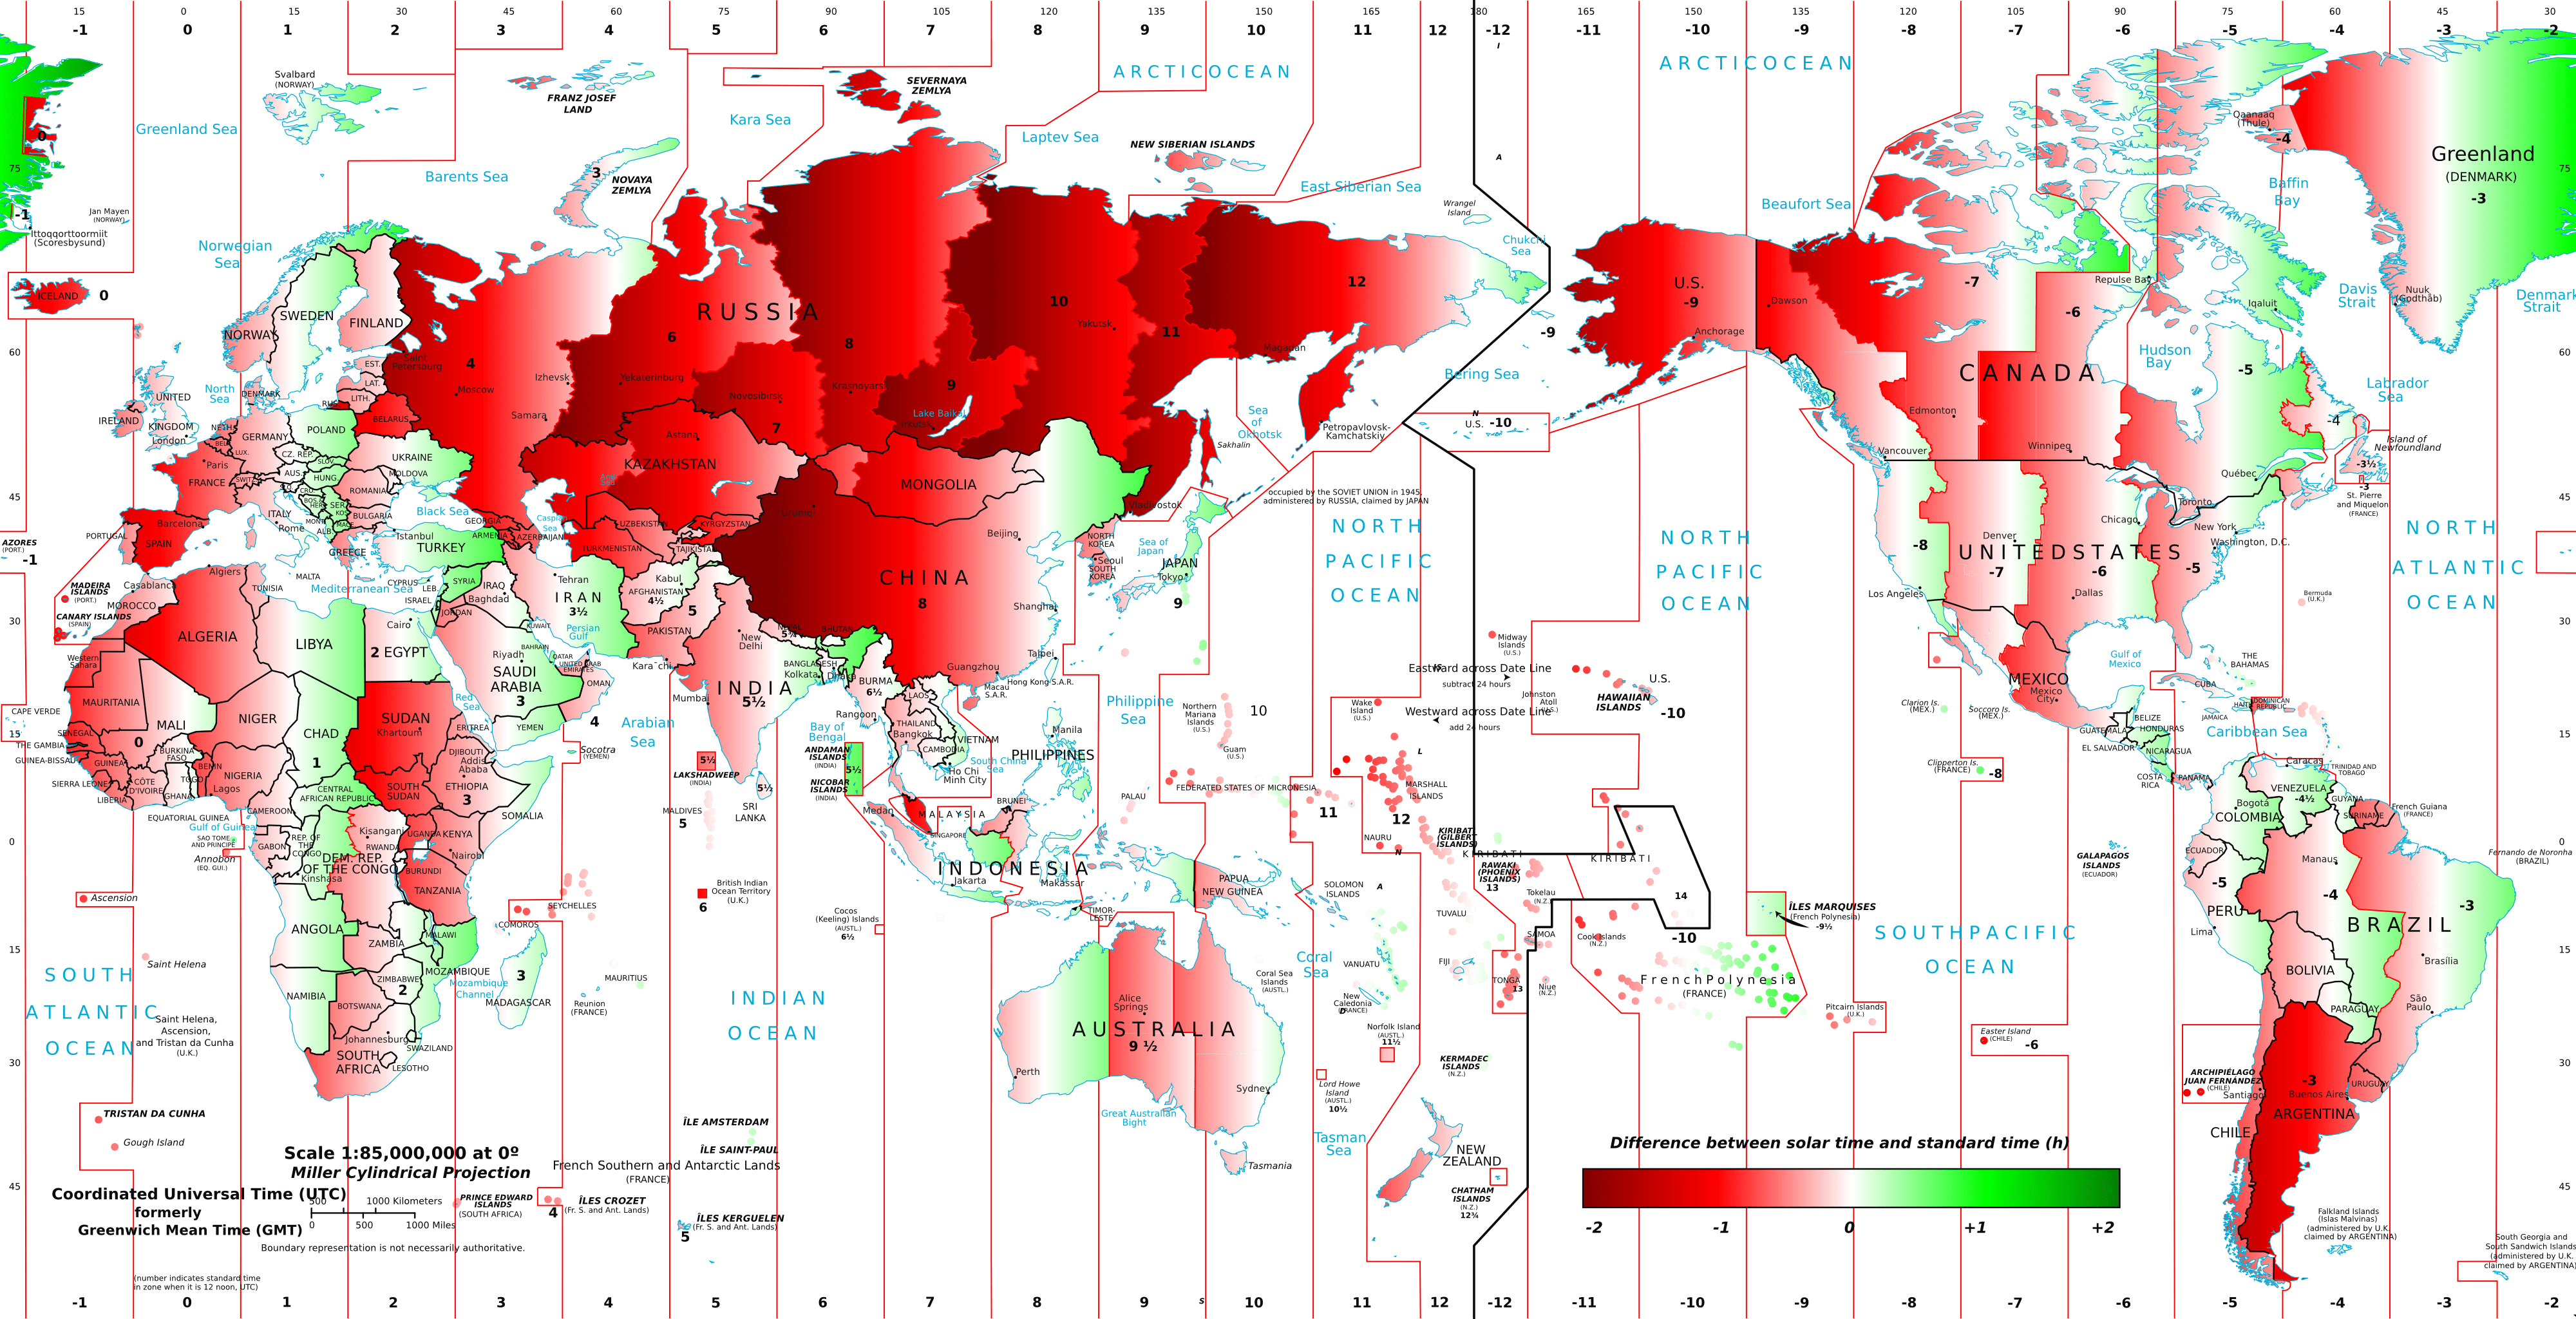
\includegraphics[width=1\textwidth]{figures/pembagian_waktu_dunia.PNG}}
\caption{menjelaskan tentang zona waktu pada tiap belahan dunia.}
\label{pembagian_waktu_dunia}
\end{figure}

Pada gambar \ref{pembagian_waktu_dunia} menjelaskan tentang zona waktu pada tiap belahan dunia.

	Perbedaan GMT dengan waktu pertengahan setempat di luar Greenwich adalah tergantung besar kecilnya Garis Bujur (BB/BT) dan dapat dirumuskan 
sebagai berikut:
\begin{equation}
WP x = GMT + BT, 
\end {equation}
atau 
\begin{equation}
WP x = GMT – BB
\end {equation}

\begin{equation}
GMT = WP x - BT, 
atau
\end{equation}
\begin{equation}
GMT = WP x + BB
\end{equation}
Contohnya sebagai berikut:

\begin {enumerate}
\item
Diketahui BT Semarang = 110° 26’
Pada saat GMT menunjukkan pukul 11.30, 
\begin{equation}
WP x = WP Semarang = 11.30 + 110° 26’
= 11.30 + 7 j 21m 44dt
= 18 j 51 m 44 dt
\end{equation}

\item
Diketahui BT Semarang = 100° 26’
Pada saat WP Semarang menunjukkan pukul 19.54,
\begin{equation}
GMT = 19.54 - 100° 26’
    = 19.54 - 8 j 24m 0dt
    = 11.30
\end{equation}
\end {enumerate}

\cite {khusurur2016mengenal}

\subsection {Dampak wilayah yang dilalui oleh garis khatulistiwa}

	Menurut sebuah artikel dari Yanti, Ari Hepi and Dhewiyanty, Varla and Setyawati, Tri Rima yang menyebutkan bahwa daerah yang dilalui garis khatulistiwa 
memiliki iklim tropis dengan suhu udara cukup tinggi dan kelembaban yang tinggi. Contoh daerah yang dilalui garis khatulistiwa yaitu Kalimantan Barat
suhu udara di Kalimantan Barat pada tahun 2013 berkisar antara 21,5oC-34,3oC (BPS Kalbar, 2014). \cite {yanti2015prevalensi}

	Masih ada lagi beberapa negara yang dilalui oleh garis khatulistiwa yang terdapat pada gambar \ref{tabel_negara_yang_dilalui_garis_khatulistiwa}

\begin{figure}[ht]
\centerline{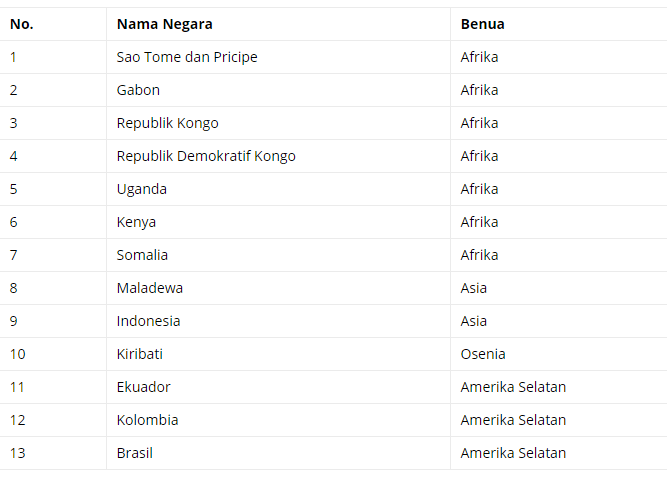
\includegraphics[width=1\textwidth]{figures/tabel_negara_yang_dilalui_garis_khatulistiwa.PNG}}
\caption{list negara yang dilalui garis khatulistiwa.}
\label{tabel_negara_yang_dilalui_garis_khatulistiwa}
\end{figure}

	Pada gambar \ref{tabel_negara_yang_dilalui_garis_khatulistiwa} disebutkan negara - negara yang dilalui oleh garis khatulistiwa yaitu Sao Tome dan Pricipe 
yang terdapat pada benua Afrika, Gabon yang terdapat di benua Afrika, Republik Kongo yang terdapat di benua Afrika, Republik Demokratif Kongo yang terdapat 
di benua Afrika, Uganda yang terdapat di benua Afrika, Kenya yang terdapat di benua Afrika, Somalia yang terdapat di benua Afrika, Maladewa yang terdapat 
di benua Asia, Indonesia yang terdapat di benua Asia, Negara Kiribati , Ekuador yang terdapat di benua Amerika Selatan, Kolombia 
yang terdapat di benua Amerika Selatan, dan Brasil yang terdapat di benua Amerika Selatan
	
	untuk lebih detailnya terdapat pada gambar \ref{Peta_Dunia_Negara_Khatulistiwa}
	
\begin{figure}[ht]
\centerline{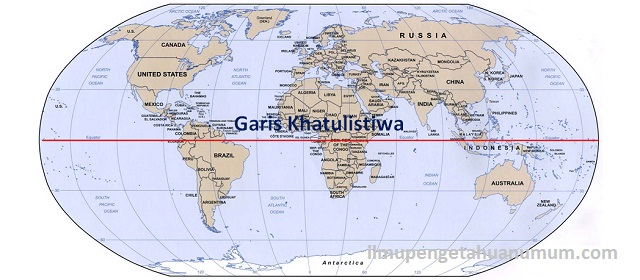
\includegraphics[width=1\textwidth]{figures/Peta_Dunia_Negara_Khatulistiwa.JPG}}
\caption{wilayah di dunia yang dilewati garis khatulistiwa.}
\label{Peta_Dunia_Negara_Khatulistiwa}
\end{figure}

\subsubsection {Peristiwa Equinox}

	Dalam sebuah artikel dari Mutoha Arkanudin yang menyebutkan bahwa selama setahun Matahari berubah posisi dari Utara ke Selatan dan sebaliknya. 
Posisi tersebut sering disebut sebagai Gerak Musim Matahari. Equinox adalah saat dimana posisi matahari berada tepat di Ekuator atau garis katulistiwa. 
Ini adalah bagian dari siklus tahunan pergerakan harian semu matahari saat terbit, melintas dan terbenam yang disebabkan oleh kemiringan sumbu bumi
terhadap bidang orbitnya yaitu sebesar 66.56 derajat. Selama setahun terjadi dua kali Equinox yaitu Maret Equinox yang terjadi setiap tanggal 21 Maret dan September
Ekuinox yang terjadi setiap tanggal 23 September. 

	Saat terjadi peristiwa Equinox posisi Matahari terbenam akan tepat berada di titik Barat sehingga dengan menambah sudut kemiringan arah kiblat 
terhadap titik Barat maka arah kiblat yang sesungguhnya kan kita dapatkan. 

	Selain Equinox matahari juga akan berada di titik paling Utara pada 21 Juni dan berada di titik paling Selatan pada 22 Desember yang dikenal dengan 
istilah Solstice. Pada saat Juni Solstice, Matahari akan terbenam tepat di sudut serong terhadap arah Barat sebesar 23,5 derajat ke arah Utara
sehingga untuk menuju ke arah kiblat yang tepat dapat tinggal menambahkan kekurangan penyerongan angka arah kiblat yang didapatkan dari hasil perhitungan 
menggunakan rumus segitiga bola. Sedangakan pada saat Desember Solstice matahari terbenam di Selatan titik Baratsebesar 23,5 derajat.\cite {arkanudin2008teknik}.

\section {Penutup}

\subsection{Kesimpulan}
	
	Garis khatulistiwa merupakan garis lintang dari 0 derajat sampai dengan 90 derajat di kutub bumi. Prime meridian atau meridian Greenwich adalah 
nilai koordinat garis bujur dimulai dari bujur 0 derajat yaitu di Greenwich, kemudian membesar ke arah timur dan barat sampai bertemu kembali di Garis batas 
internasional yaitu terletak di Selat Bering dengan nilai 180 derajat. Sistem koordinat dimaksudkan untuk memberikan pengalamatan terhadap setiap lokasi 
di permukaan bumi. Meridian Utama atau Prime Meridien digunakan untuk menentukan waktu di dunia, metode penentuan mengikuti Waktu Universal (bahasa 
Inggris Universal Time, disingkat UT) adalah satu ukuran waktu yang didasari oleh rotasi bumi. daerah yang dilalui garis khatulistiwa memiliki iklim tropis 
dengan suhu udara cukup tinggi dan kelembaban yang tinggi.

\subsection{Saran}

	Dalam artikel ini belum ada penjelasan mengenai sejarah garis khatulistiwa dan prime meridien, maka diharapkan untuk  kedepannya dilengkapi dengan 
informasi mengenai sejarah dari garis khatulistiwa dan prime meridien.	


\chapter[Kordinat Indonesia]
{Pengantar\\ Kordinat Indonesia}
% Nama kelompok : 3
% Kelas : D4 Teknik Informatika 3C
% 1. Kezia Tirza Naramessakh (1154093)
% 2. Mariani Rospilinda Siki (1154107)
% 3. Doli Jonviter Nt Simbolon (1154016)
% 4. Benedictus Simantupang (1154116)
% 5. Dimas Mathovani 


\section{Koordinat Lintang Utara, Lintang Selatan, Bujur Timur, Bujur Barat}
Koordinat digunakan untuk menunjukkan suatu titik di Bumi berdasarkan garis lintang dan garis bujur. Koordinat dibagi menjadi dua bagian irisan yaitu irisan melintang yang disebut dengan garis lintang mulai dari khatulistiwa, membesar ke arah kutub(utara maupun selatan) sedangkan yang lain membuju r mulai dari garis Greenwhich membesar ke arah barat dan timur. Satuan skala koordinat dibagi dalam derajat lintang 0* sampai 90* dan bujur 0* sampai 180*. Koordinat ini ditulis dalam satuan derajat, menit, dan detik, misalnya 110*35'32", dan seterusnya. Untuk membagi dunia dalam wilayah utara dan selatan, maka ditentukan sebuah garis yang tepat berada di tengah, yaitu garis Equator / Khatulistiwa. Untuk membagi wilayah timur dan barat, maka ditentukan sebuah garis Prime meridian yang terletak di kota Greenwich (Inggris), dan perpotongannya bertemu di wilayah laut pasific, yakni memotong kepulauan Fiji.
Koordinat pada gambar \ref{Koordinat} di jelaskan garis Lintang dan Bujur
\begin{figure}[ht]
	\centerline{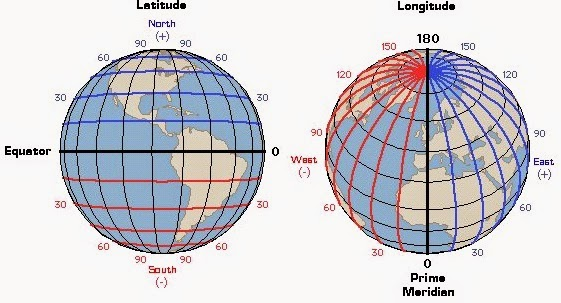
\includegraphics[width=1\textwidth]{figures/Koordinat.JPG}}
	\caption{Koordinat Lintang dan Bujur}
	\label{Koordinat}
	\end{figure}

\subsection{Sistem Koordinat}
Dalam artikel Zuhdi menjelaskan Koordinat dimaksudkan untuk memberikan pengalamatan terhadap setiap lokasi di permukaan bumi. Pengalamatan dengan sistem koordinat didasarkan atas jarak timur-barat dan utara-selatan suatu tempat dari suatu titik pangkal tertentu. Jarak diukur dalam satuan derajat sudut yang dibentuk dari titik pangkal ke posisi tersebut melalui pusat bumi. Sedangkan titik pangkal ditetapkan berada di perpotongan belahan utara-selatan bumi (garis khatulistiwa) dengan garis yang membelah bumi timur-barat melalui kota GreenWhich di Inggris. 
Untuk lebih jelas tentang bentuk titik koordinat lihat pada gambar \ref{sistemkoordinat} dibawah ini :
\begin{figure}[ht]
	\centerline{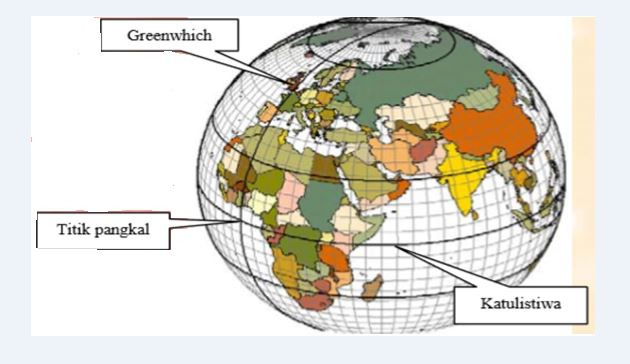
\includegraphics[width=1\textwidth]{figures/sistemkoordinat.JPG}}
	\caption{Bentuk titik Koordinat}
	\label{sistemkoordinat}
	\end{figure}

Baik garis lintang maupun garis bujur diukur dalam derjat dan dibagi lagi dalam menit dan detik. 1 derajat garis bujur diukur lapangan sama dengan 11,32 km. Satuan derajat bisa juga disebut jam sehingga setiap derajat terbagi menjaid 60 menit dan setiap menit terbagi menjadi 60 detik. Dalam penulisan letak astronomis contohnya 60 derajat 23' 15"S, maka dibaca sebagai 60 derajat 23 menit 15 detik lintang selatan. pada sistem pemetaan internasional huruf U sebagai lintang utara diganti dengan huruf N (north). Besar sudut dalam sistem koordinat geografik dapat dinyatakan dalam dua cara, yaitu dengan satuan DMS(Degree Minute Second) atau satuan DD(Decimal Degree), dalam sistem satuan DMS, setiap derajat sudut dibagi menjadi 60 menit dan setiap menitnya dibagi lagi menjadi 60 detik. Penulisannya dinyatakan sebagai dd°mm'ss". Sedangkan pada sistem satuan setiap derajatnya dinyatakan dalam pecahan decimal (pecahan berkoma). Baik dalam DMS maupun DD, perlu diketahui berapa ketelitian suatu nilai koordinat. Karena di wilayah khatulistiwa jarak 1° sama dengan jarak 111321 meter. Maka perlu diperhatikan keselahan yang terjaddi jika kita mengabaikan suatu angka menit atau detik pada DMS atau suatu nilai digit dalam koordinat DD. Pada sistem DD, perlu diperhatikan jarak yang diwakili oleh setiap digit dibelakang koma. Perubahan satu satuan padaa digitt pertamma dii belakang koma mempunyai nilai jarak lebih dari 11 Km. Perubahan satu unit pada digit keduat dibelakang koma berarti 1,1 Km. Demikian seterusnya. Berarti jika kita misalnya hanya mentolerir kesalahan sampai 100 m, maka koordinat DD harus dibuat setidaknya sampai 4 digit di belakang koma. Kombinasi antara garis lintang dan garis bujur akan membentuk sutau koordinat lokasi di permukaan bumi dengan sumbu x sebagai garis lintang dan sumbu y sebagai garis bujur dalam koordinat kartesius. Pada Bujur/Longitude (X) merupakan garis yang perpindahannya secara vertical dan pada Lintang/Lattitude (Y) merupakan garis yang mempunyai perpindahan secara horizontal. \cite{zuhdi2012sistem}.

Lihat pada gambar \ref{lintangbujur} dibawah ini :
\begin{figure}[ht]
	\centerline{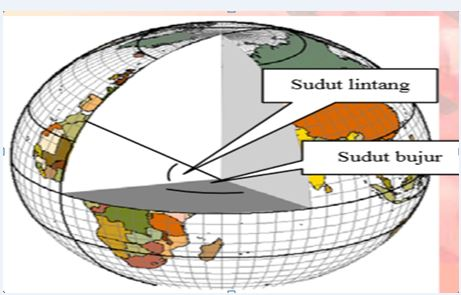
\includegraphics[width=1\textwidth]{figures/lintangbujur.JPG}}
	\caption{Titik Lintang dan Bujur}
	\label{lintangbujur}
	\end{figure}

\subsubsection{Garis Lintang}
Sebuah garis khayal yang digunakan untuk menentukan lokasi di Bumi terhadap garis khatulistiwa(utara atau selatan). Posisi lintang merupakan penghitungan sudut dari 0 derajat di khatulistiwa sampai ke +90 derajat di kutub utara dan -90 derajat di kutub selatan. Dalam bahasa indonesia lintang di sebelah utara khatulistiwa diberi nama Lintang Utara(LU), demikian pula lintang di sebelah selatan khatulistiwa diberi nama Lintang Selatan(LS). Lintang Utara dan Lintang Selatan menyatakan besarnya sudut antara posisi lintang dengan garis Khatulistiwa. Garis Khatulistiwa sendiri adalah lintang 0 derajat. 
Nilai koordinat lingtang dimulai dari garis lingkaran khatulistiwa yang diberi nilai 0 derajat. Selanjutnya garis lintang yang lain berupa lingkarang paralel (sejajar) katulistiwa berada disebelah utara dan selatan khatulistiwa. Lingkaran paralel di selatan disebut garis lintang selatan (LS) dan diberi nilai negatif, sedangkan lingkaran paralel diutara diberi nilai positif dan disebut garis lintang utara (LU). Nilai maksimum koordinat garis lintang adalah 90 derajat yaitu terletak di kutub-kutub bumi. 
Lingkaran paralel merupakan representasi garis lintang ini semakin mengecil ukurannya dengan semakin jauh dari katulistiwa. sehingga jarak 1 derajat timur-barat dari katulistiwa jauh lebih besar dari pada jarak 1 derajat timur-barat di tempat yang jauh dari katulistiwa. Di khtulistiwa 1 derajat timur-barat sama dengan 111.321 km, tapi di dekat kutub 1 derajat timur-barat hanya beberapa meter saja. itu sebabnya grid yang dibuat dari garis lintang dan garis bujur, tampak berupa sangkar dikatulistiwa dan berubah menjadi persegi didaerah kutub
lintang memiliki symbol phi dan menunjukkan sudut antara garis lurus dititik tertentu dengan bidang ekuator. Lintang ditentukan dalam angka derajat dimulai dari 0 derajat dan berakhir dengan 90 derajat. garis lintang ini membagi bumi menjadi belahan bumi utara dan selatan. garis ekuator atau khatulistiwa berada di lintang 0 derajat. Garis lintang biasa digunakan untuk melihat penyebaran iklim di bumi.
Latitude aau garis lintang adalah garis yang menentukan lokasi berada di sebelah utara atau selatan ekuator. garis lintang diukur mulai dari titik 0 derajat dari khatulistiwa sampai 90 derajat di kutub. Garis lintang digunakan untuk membatasi corak iklim di permukaan bumi, berikut ini merupakan pembagian iklim di bumi menurut batas garis lintang:
1. 23,5-23,5 LU/LS = iklim tropis
2. 23,5-40 LU/LS = iklim subtropis
3. 40 Lu-66,5 LU/LS = iklim sedang
4. 66,5-90 LU/LS = iklim kutub
Indonesia terletak antara 6 derajat Lintang Utara (LU) – 11 derajat Lintang Selatan (LS) dan diantara 95 derajat bujur timur – 141 derajat Bujur timur.
Adapun wilayah indonesia itu pada bagian paling utara yang ebrada di Pulau Weh di Nanggroe Aceh Darussalam yang terletak pada 6 derajat lintang utara, dan untuk daerah indonesia yang paling berada di selatan yaitu Pulau Roti di Nusa Tenggara Timur yang terletak pada 11 derajat lintang selatan. Kemudian mengacu pada letak lintangnya, di wilayah Indonesia berada pada 6 derajat lintang utara – 11 derajat lintang selatan, hal tersebut disebabkan indonesia mempunyai iklim tropis dengan beberapa ciri-ciri yaitu mempunyai hutan hujan tropis yang begitu luas dan mempunyai nilai ekonomis yang sangat tinggi, mendapatkan sinar matahari yang lama setiap sepanjang tahun, mempunyai curah hujan yang tinggi dan memiliki banyak penguapan sehingga akan meningkatkan kelembaban udara.
Pada gambar \ref{lintang} dijelaskan titik koordinat Lintang pada sumbuh Y :
\begin{figure}[ht]
	\centerline{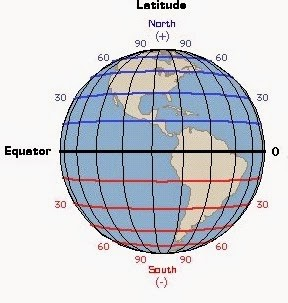
\includegraphics[width=1\textwidth]{figures/lintang.JPG}}
	\caption{Titik koordinat Lintang pada sumbuh Y}
	\label{lintang}
	\end{figure}

\subsubsection{Garis Bujur}
Menggambarkan lokasi sebuah tempat di timur atau barat Bumi dari sebuah garis utara-selatan yang disebut Meridian Utama. Longitude diberikan berdasarkan pengukuran sudut yang berkisar dari 0 derajat Meridian Utama ke +180 derajat arah timur dan -180 derajat arah barat. Tidak seperti lintang yang memiliki ekuator sebagai posisi awal alami, tidak ada posisi awal alami untuk bujur. Bujur di sebelah barat Meridian diberi nama Bujur Barat(BB), demikian pula bujur di sebelah timur Meridian diberi nama Bujur Timur(BT).
Nilai koordinat garis bujur dimulai dari bujur 0 derajat yaitu Greenwhich, kemudian memebersasr ke arah timur dan barat sampai bertemu kembali di garis batas tanggal internasional yaitu terletak di selat bering dnegan nilai 180 derajat. garis bujur 0 derajat disebut prime meridian atau meridian greenwhich. garsi bujur ke arah barat diberi nilai negatif dan disebut bujur barat (west longitude) serta disingkan BB. sedangkan garis bujur yang ke arah timur diberi nilai positif dan disebut bujur timur (east longitude) disingkat BT. nilai koordinatnya didasarkan atas besarnya sudut yang terbentuk dari bujur 0 ke garis bujur tersebut melalui pusat bumi.
Longitude atau garis bujur memiliki symbol lamda. garis bujur ini merupakan garis yang menunjukkan bagian barat dan timur dilihat dari titik pangkal yaitu di greenwich meridian. garis bujur emiliki batas maksimum yaiu 180 derajat ke arah timur dar GMT dan 180 derajat ke arah barat dari GMT. keduanya bertemu di garis internasional date line disekitar pasifik.
longitude atau garis bujur digunakan untuk menentukan lokasi diwilayah barat atau timur dari garis utara selatan yang sering disebut juga garis meridian. garis bujur digunakan untuk menentukan waktu dan tanggal.
Titik di barat bujur 0° dinamakan Bujur Barat sedangkan titik di timur 0° dinamakan Bujur Timur. Kombinasi garis lintang dan garis bujur ini berguna untuk menentukan suatu lokasi di permukaan bumi. Garis Lintang menandakan sumbu y dan garus bujur menandakan sumbu x dalam sistem koordinat cartesian. Sebagi contoh kota Sabang di pulau We berada pada koordinat 6oLU 95o BT, dan kota Merauke di Papua memiliki koordinat 11oLS dan 141oBT.
Indonesia berada pada 95 derajat bujur timur – 141 derajat bujur timur menyebabkan Indonesia mempunyai tiga waktu dan pada setiap waktu memiliki daerah tersendiri, sehingga Indonesia memiliki beberapa pembagian waktu yaitu Waktu Indonesia bagian timur atau WIT mencakup Papua, kepulauan Maluku dan pulau-pulau kecil disekitarnya. Untuk waktu indonesia bagian  timur mempunyai selisih waktu sebanyak 9 jam lebih awal dari Greenwich Mean time atau GMT. Kemudian untuk Waktu Indonesia bagian tengah atau WITA mencakup Nusa tenggara, kalimantan selatan, Pulau Sulawesi, Bali dan pulau-pulau kecil yang ada disekitarnya. Untuk Indonesia bagian tengah mempunyai selisih waktu sebanyak 8 jam yang lebih awal dari Greenwich mean time (GMT). Kemudian, untuk daerah waktu Indonesia bagian barat atau WIB yang mencakup Madura, Jawa, kalimantan barat, kalimantan tengah, Sumatera dan pulau-pulau kecil yang ada disekitarnya. Adapun waktu indonesia bagian barat mempunyai selisih waktu sebanyak 7 jam yang lebih awal dari Greenwich mean time.
Pada gambar \ref{bujur} dijelaskan titik koordinat Lintang pada sumbuh X :
\begin{figure}[ht]
	\centerline{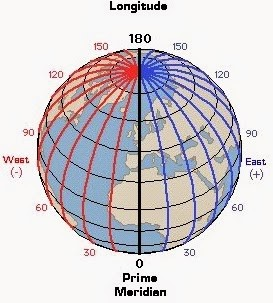
\includegraphics[width=1\textwidth]{figures/bujur.JPG}}
	\caption{Titik koordinat Bujur pada sumbuh X}
	\label{bujur}
	\end{figure}

\chapter[Kordinat Internasional]
{Pengantar\\ Kordinat Internasional}
% Nama Kelompok 2 : Latitude & Longitude
% Kelas : D4TI3C
% Adhika Dwi Cahya Putra (1154017)
% Haris Munandar Alwi (1154105)
% Muhammad Adam Nahdlotul Halimi (1154024)
% Tito Aryo Nugroho (1154074)
% Tomy Prawoto (1154121)

\section{latitude longitude}

\subsection{Latitude}
Latitude merupakan terjemahan bahasa inggris dari garis lintang. Garis lintang dapat disebut juga sebagai garis khatulistiwa (0 derajat), atau bisa disebut juga sebagai garis tengah bumi yang membagi antara belahan bumi bagian atas dan bumi bagian bawah.
Dalam sebuah buku karangan Maling \& Derek Hylton yang berjudul \"Coordinate System and Map Projections\" mengatakan bahwa garis lintang suatu titik dapat didefinisikan secara formal sebagai sudut yang diukur di tengah bumi di antara bidang equator dan jari jari yang ditarik ke titik. 
Pada garis lintang bagian utara bumi dilambangkan dengan tanda \verb|'+phi'| 
sedangkan garis lintang bagian selatan bumi dilambangkan dengan tanda \verb|'-phi'| 
\cite{maling2013coordinate}. 

	\begin{figure}[ht]
	\centerline{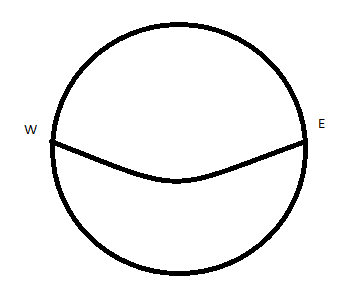
\includegraphics[width=1\textwidth]{figures/latitude.PNG}}
	\caption{Garis Lintang atau Latitude.}
	\label{latitude}
	\end{figure}
Pada gambar \ref{latitude} merupakan gambar latitude atau garis lintang yang membentang antara west(barat) sampai east(timur).
Garis lintang digunakan sebagai penanda dalam zona iklim di dunia. Dari +23 setengah derajat Lintang Utara sampai -23 setengah Lintang Selatan memiliki zona iklim tropis. Zona iklim tropis hanya memiliki dua musim, yaitu kemarau atau panas dan penghujan saja. Kemudian dari +23 setengah derajat Lintang utara sampai +66 setengah derajat Lintang utara memiliki zona iklim subtropis. Sama halnya bagian utara, bagian selatan yaitu -23 setengah derajat lintang selatan sampai -66 setengah derajat lintang selatan memiliki zona iklim subtropis. Daerah subtropis memiliki 4 musim, yaitu spring, summer, fall, dan winter. 

\subsection{Longitude}
Longitude merupakan terjemahan bahasa inggris dari garis bujur. Garis bujur biasa digunakan untuk menentukan waktu dan tanggal di dunia yang kita huni sekarang ini. Jika garis lintang atau latitude atau daerah khatulistiwa dianggap sebagai 0 derajat, maka garis bujur merupakan 0 derajat yang menghubungkan kutub utara dengan kutub selatan yang melawati kota Greenwich di Inggris. Garis bujur bagian barat kota Greenwich disebut sebagai Bujur Barat sedangkan garis bujur yang berada pada sebelah timur kota Greenwich disebut sebagai Bujur Timur. Inilah penyebab kenapa orang indonesia disebut sebagai orang timur.
	\begin{figure}[ht]
	\centerline{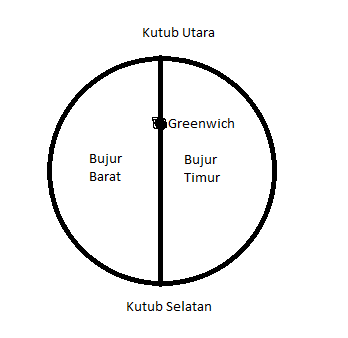
\includegraphics[width=1\textwidth]{figures/longitude.PNG}}
	\caption{Garis Bujur atau Longitude.}
	\label{longitude}
	\end{figure}
Pada gambar \ref{longitude} merupakan gambar longitude atau garis bujur yang menghubungkan kutub utara dengan kutub selatan. Garis ini melewati kota Greenwich di Inggris.
Garis bujur digunakan untuk pembagian zona waktu di dunia.

\section{LINTANG}

	Sudut lintang l
	Bayangkan Bumi adalah bola transparan (sebenarnya
	bentuknya agak oval; karena rotasi bumi, nya
	Khatulistiwa sedikit menonjol). Melalui Bumi yang transparan
	(gambar) kita bisa melihat bidang ekuatornya, dan bagian tengahnya
	titik adalah O, pusat bumi.
	Untuk menentukan garis lintang beberapa titik P di permukaan, tariklah
	radius OP ke titik itu. Maka sudut elevasi titik itu
	Di atas garis ekuator adalah garis lintang l - lintang utara jika utara
	dari garis khatulistiwa, lintang selatan (atau negatif) jika selatannya.
	Garis lintang. Di dunia bumi, garis lintang adalah lingkaran dengan ukuran yang berbeda. Itu
	terpanjang adalah khatulistiwa, yang garis lintangnya nol, sementara di kutub - di garis lintang
	90 ° utara dan 90 ° selatan (atau -90 °) lingkaran menyusut ke titik tertentu.

\section{GARIS BUJUR}
	Di dunia, garis bujur konstan ("meridian") meluas dari tiang ke kutub, seperti
	batas segmen pada jeruk kupas.
	Garis bujur atau "garis meridian"
	Setiap meridian harus melewati garis khatulistiwa. Karena ekuator adalah lingkaran, kita bisa
	bagilah itu - seperti lingkaran - ke dalam 360 derajat, dan bujur f dari sebuah titik adalah
	maka nilai yang ditandai dari divisi mana meridiannya memenuhi khatulistiwa.
	Apa nilai itu tergantung tentu saja dari mana kita mulai menghitung - di mana
	nol bujur adalah Untuk alasan historis, garis meridian melewati Astronomi Kerajaan yang lama
	Observatorium di Greenwich, Inggris, adalah yang dipilih sebagai nol bujur. Bertempat di Jl
	Tepi timur London, ibu kota Inggris, observatorium sekarang menjadi museum umum dan a
	band kuningan yang membentang di halamannya menandai "garis meridian utama". Wisatawan sering mendapatkan
	difoto saat mereka mengangkangnya - satu kaki di belahan bumi bagian timur, yang lainnya masuk belahan barat.
	Garis bujur juga disebut meridian, berasal dari bahasa Latin, dari meri, a
	variasi "medius" yang menunjukkan "tengah", dan diem, yang berarti "hari". Kata itu
	pernah berarti "siang", dan waktu sehari sebelum siang hari dikenal sebagai "ante meridian",
	sementara waktu setelah itu adalah "posting meridian." Singkatan hari ini a.m. dan p.m. datang
	Dari istilah ini, dan Matahari pada siang hari dikatakan "melewati meridian". Semua poin di
	garis bujur yang sama mengalami siang hari (dan jam lainnya) pada saat bersamaan dan
	oleh karena itu dikatakan sama "garis meridian", yang menjadi "meridian" untuk
	pendek.

\section{Waktu Lokal (LT) dan Zona Waktu}
	Garis bujur diukur dari nol sampai 180 ° BT dan 180 ° BB (atau -180 °), dan kedua 180-
	Gelombang longitudinal berbagi jalur yang sama, di tengah Samudera Pasifik.
	Saat Bumi berputar mengelilingi porosnya, kapanpun satu garis bujur - "siang hari
	meridian "- menghadap Matahari, dan pada saat itu, akan ada siang hari di mana-mana di atasnya
	jam Bumi telah mengalami rotasi penuh sehubungan dengan Matahari, dan meridian yang sama
	lagi wajah siang hari Jadi setiap jam Bumi berputar 360/24 = 15 derajat.
	Bila di lokasi Anda waktu 12 siang, 15 ° ke timur waktu adalah 1 p.m., karena itu adalah
	meridian yang dihadapi Matahari sejam yang lalu. Di sisi lain, 15 ° ke barat waktu adalah 11
	a.m., untuk satu jam lagi, meridian itu akan menghadapi Matahari dan mengalami siang hari.

\subsection{Glosarium}
	Khatulistiwa-Garis yang mengelilingi Bumi pada jarak yang sama dari Utara dan Selatan
	Polandia Koordinat geografis - Koordinat nilai yang diberikan sebagai garis lintang dan bujur.
	Lingkaran besar - Sebuah lingkaran terbentuk di permukaan bola oleh sebuah pesawat yang melewati
	pusat bola. Khatulistiwa, masing-masing meridian, dan satu sama lain keliling penuh
	Bumi membentuk lingkaran besar. Arus lingkaran besar menunjukkan jarak terpendek antara titik-titik di permukaan bumi.

	\subsubsection{Meridian}
	Lingkaran besar di permukaan Bumi, melewati kutub geografis
	dan beberapa titik ketiga di permukaan bumi. Semua poin pada meridian tertentu memiliki hal yang sama
	\subsubsection{Paralel}
	Lingkaran atau perkiraan lingkaran di permukaan Bumi, sejajar dengan
	Khatulistiwa dan titik penghubung dengan garis lintang yang sama.
	\subsubsection{Prime Meridian}
	Garis meridian bujur 0 derajat, digunakan sebagai asal untuk
	pengukuran bujur. Garis meridian Greenwich, Inggris, adalah internasional
	menerima meridian utama dalam banyak kasus.

\section{Konversi antara koordinat geografis dan cartesian koordinat}
	Asumsikan bahwa koordinat geografis dari suatu titik M adalah l dan f; asumsikan bahwa jari - jari
	Bumi adalah R. Masalahnya adalah penentuan koordinat kartesius M dalam a
	Sistem koordinat asal pusat bumi, dengan bidang horisontal xoy bidang
	Khatulistiwa, dengan sumbu x melewati meridian Greenwich, sumbu y secara langsung
	tegak lurus dengan sumbu x, dan akhirnya sumbu z melewati kutub.
	Tujuannya adalah untuk menemukan x, y dan z.

	Tunjukkan pada gambar sudut l dan f;
	Berapakah jarak OM?
	Hitung jarak OH menurut l.
	Berapakah nilai x dan y menurut l dan f;
	Berapakah nilai z?
	Asumsikan bahwa koordinat geografis dari suatu titik V
	adalah:
	garis lintang: 45 ° 41'47.59 '' N
	Bujur: 4 ° 52 '+ 49,98' 'E
	Apa koordinat kartesian V (dengan R = 1)
	Sebenarnya, titik ini persis sekolah kita!

\section{LINTANG/LATITUDE}

	Latitude adalah garis mendatar. Titik 0 adalah sudut ekuator tanda + menunjukan arah ke atas menuju kutub utara,
	sementara tanda minus di koordinat menuju ke kutub selatan. Bayangkan bila bumi hanyalah sebuah bola transparan 
	(sebenarnya bentuk bumi adalah oval; ini dikarenakan rotasi bumi itu sendiri, karena garis khatulistiwa sedikit 
	terlihat). Dengan bumi yang transparan, kita bisa lihat (gambar)
	\begin{figure}[ht]
	\centerline{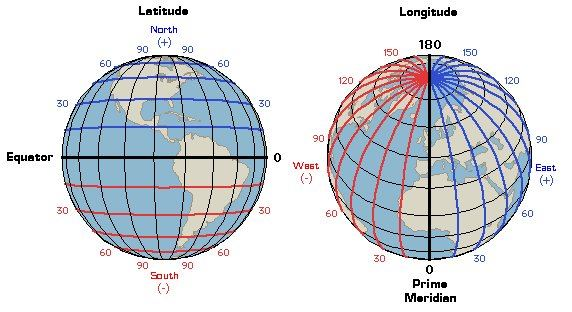
\includegraphics[width=1\textwidth]{figures/Latitude.jpg}}
	\caption{gambar Latitude.}
	\label{Gambar Latitude}
	\end{figure}
	garis khatulistiwa bumi, dan garis tengahnya adalah
	0, pusat bumi. Untuk menentukan latitude ( garis lintang ) dibeberapa titik P di permukaan, buatlah suatu jarak OP 
	ke suatu titik. Lalu sudut elevasi titik tersebut berada diatas garis ekuator adalah garis lintang l - lintang utara
	jika dari utara, lintang selatan ( negatif ) jika dari selatan. 
	Garis Lintang, dalam bola bumi, garis lintang dalam lingkaran memiliki perbedaan ukuran. Garis paling panjang adalah 
	Khatulistiwa, dimana yang lintangnya 0 ( nol ), sementara di daerah kutub, garis lintangnya 90° utara dan 90° selatan
	( atau bisa juga -90°) lingkarannya menyusut ke titik tertentu.

\section{BUJUR/LONGTITUDE}

	Longtitude adalah garis bujur, dimana garis bujur ini diawali dari titik 0° sampai 180° ke arah sebaliknya. Titik 0° dimulai dari
	garis negara Inggris, mengarah ke Indonesia akan menjadi angka positif. Jika koordinat longitude ( lintang ) akan menjadi minus 
	kearah kebalikan. Di bola bumi, garis bujur konstan meluas dari kutub ke kutub seperti batas segmen pada jeruk kupas. Garis Bujur atau
	Meridian ( gambar )
	\begin{figure}[ht]
	\centerline{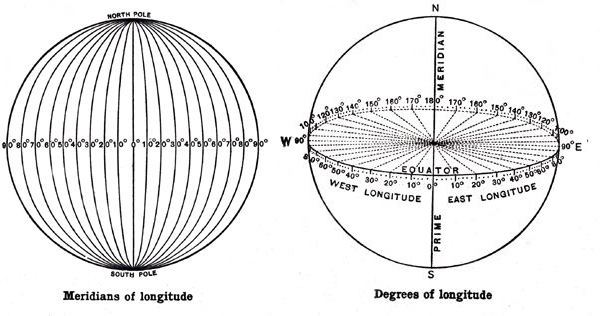
\includegraphics[width=1\textwidth]{figures/Longitude.jpg}}
	\caption{gambar longitude.}
	\label{Gambar Longitude}
	\end{figure}
	
	Setiap meridian harus menyberangi garis khatulistiwa. Karena khatulistiwa adalah sebuah lingkaran, kita bisa membagi nya seperti lingkaran
	yang lain ke dalam 360°,dan garis bujur f dari sebuah titik yang ditandai dimana meridian bertemu khatulistiwa.
	Nilai tersebut tentu bergantung pada saat kita mulai menghitung titik 0° garis bujur. Untuk alasan sejarah, garis bujur melewati Old Royal -
	Astronomical Obsevatory di Greenwich, Inggris, dimana garis 0° bujur di tetapkan. Berlokasi di tepi timur inggris, ibukota Inggris, Observatorium
	sekarang adalah Museum Umum dan suatu tanda yang membentang diatas halamannya yang menandai sebagai "garis meridian utama".
	Garis bujur atau dengan nama lain meridian, berasal dari bahasa latin, yaitu meri, variasi dari "merius" yang berarti "tengah" dan diem yang berarti 
	"hari". Kata tersebut juga bisa berarti "sore", dan waktu pada satu hari sebelum sore kita sebut sebagai "ante meridian" dimana waktu setelahnya berarti 
	"post meridian".Pada saat ini disingkat menjadi a.m. dan p.m. yang berasal dari istilah ini, dan matahari pada saat menjelang malam hari disebut sebagai
	"passing meridians". Semua titik pada setiap garis yang sama dalam garis bujur disebut sore ( dan pada jam lainnya ) pada saat yang sama dan oleh karena 
	itu disebut "garis meridian", yang menjadi "meridian" untuk lebih singkat.





\bibliographystyle{IEEEtran}
\bibliography{aku,SejarahBumi,koordinatindo,definisi,longlat,BangunRuang,kartesius,benua,khatulistiwa}


\printindex
\end{document}

